% We are writing an article
\documentclass{article}
\usepackage[margin=4cm]{geometry}

% allow useage of graphics 
\usepackage[pdftex]{graphicx}
\usepackage{wrapfig}
%\usepackage[final]{graphicx}
%\usepackage[dvipdfmx]{graphicx} 
%\usepackage{bmpsize}

% Allow the usage of utf8 characters
\usepackage[utf8]{inputenc}

% The maths package
\usepackage{amsmath}
% For double line element like R, C or Z
\usepackage{amsfonts}
% For double line element like 1, 2, ..
\usepackage{dsfont}
% For is defined as symbol (coloneqq)
\usepackage{mathtools}
% for Proof paragraphs
\usepackage{amsthm}
% to enumerate with roman bulletpoints
\usepackage{enumerate}

%subitem bulletpoints
\usepackage{outlines}

% bibtex style
%\usepackage{apacite}
\usepackage{cite}

% a packages just used for the tabulator for the pascals triangle
\usepackage{array}

% package to alighn images
%\usepackage[export]{adjustbox}
\usepackage{float}
\usepackage{subcaption}

% use the tikz package, no clue why I need the positioning thing
\usepackage{tikz}
\usetikzlibrary{positioning}

\usepackage{hyperref}

% as it sais. Start the section counter from zero
% instead of starting it at one
\setcounter{section}{-1}

\theoremstyle{definition}
\newtheorem{theorem}{Theorem}[section]
\newtheorem{corollary}[theorem]{Corollary}
\newtheorem{lemma}[theorem]{Lemma}
\newtheorem{definition}[theorem]{Definition}
\newtheorem{proposition}[theorem]{Proposition}
\newtheorem{remark}[theorem]{Remark}
\newtheorem{example}[theorem]{Example}
\newtheorem{convention}[theorem]{Convention}

\DeclareMathOperator{\Conv}{Conv}
\DeclareMathOperator{\grad}{grad}
\DeclareMathOperator{\Rat}{Rat}
\DeclareMathOperator{\Pol}{Pol}
%\DeclareMathOperator{\Im}{Im}

% create a command to easyly add figure titles
\newcommand*{\figuretitle}[1]{%
    {\centering%   <--------  will only affect the title because of the grouping (by the
    \textbf{#1}%              braces before \centering and behind \medskip). If you remove
    \par\medskip}%            these braces the whole body of a {figure} env will be centered.
}

% Another new command (restr{f}{A})
\newcommand\restr[2]{{% we make the whole thing an ordinary symbol
  \left.\kern-\nulldelimiterspace % automatically resize the bar with \right
  #1 % the function
  % \vphantom{\big|} % pretend it's a little taller at normal size
  \right|_{#2} % this is the delimiter
  }}

\title{Tropical Geometry of Deep Neural Networks}
\author{David Leatham}
\date{\today}

% Start the document
\begin{document}


%\maketitle
\begin{titlepage}
	\begin{center}
		\vspace*{2.5cm}
		\begin{LARGE}
		Bachelor Thesis
		\end{LARGE}
		
		\vspace{0.3cm}
		\LARGE
		\textbf{Tropical Geometry of \\ Deep Neural Networks}
		
		\vspace{1cm}
		
		\large
		David Leatham \\
		\vspace{0.2cm}
		\large
		\today
		
	\end{center}
	
\end{titlepage}

\newpage
  
\tableofcontents

\newpage


% Create a new 0th level heading named Introduction
\section{Introduction} 
\leavevmode
\\
Tropical geometry is a modern branch of mathematics subject to a rise in research throughout the past 30 years. Neural networks have found application in many disciplines and have been used to algorithmically manage complex tasks like self driving cars, face and text recognition or automatically processing hand written checks at banks. Neural networks impact our lives on a daily basis. \\
In this thesis we describe a new representation of neural networks through tropical geometry, following the recent article "Tropical Geometry of Deep Neural Networks" by Liwen Zhang, Gregory Naitzat and Lek-Heng Lim \cite{maclagan2015introduction}. \\

The subject of neural networks was introduced by Warren McCulloch and Walter Pitts in 1943 when they created a computational model for neural networks \cite{mcculloch1943logical}. In the following years one of the next big steps towards today's state of the art neural networks, was the research into the underlying concepts of backpropagation in 1960 by Kelley \cite{kelley1960gradient} and 1961 by Bryson \cite{bryson1961gradient}. Backpropagation is an algorithm describing a key concept of training neural networks. Starting around $2010$ to this day neural networks are experiencing a boost in popularity. This is due to hardware improvements especially in GPU's making backpropagation feasible \cite{cirecsan2010deep}, the growing amount of data and the improvement of knowledge on deep neural networks fuelled by articles and works, for example that of Andrew Yan-Tak Ng and Jeff Dean in 2012. They created a network that learned to recognize higher-level concepts, such as cats, only from watching unlabeled images \cite{DBLP:journals/corr/abs-1112-6209}. Nowadays neural networks help solve challenging problems in computer science and software engineering and, in particular, they are key to application areas such as system identification and control, pattern and sequence recognition, social network filtering and e-mail spam filtering. \\

Tropical geometry on the other hand is a field of interest in mathematics, whose underlying analytical ideas have been around some years before $1990$, for example by Victor Pavlovich Maslov \cite{maslov1985new}. But only since then have there been basic efforts to consolidate the basic definitions as research increased and from $2000$ onwards gained the attention it receives nowadays carried by successful applications in enumerative tropical algebraic geometry for instance by Grigory Mikhalkin in 2005 \cite{mikhalkin2005enumerative}. 
Tropical geometry is the study of polynomials under tropical multiplication and addition, where tropical multiplication is usual addition and tropical addition of two elements returns the minimal element. It is used in mathematics itself \cite{krivulin2014tropical}, finance \cite{klemperer2009new} and computer since. For the last topic this thesis is an example, as we describe a fundamental mathematical connection between tropical geometry and deep neural networks. \\

Concerning the structure of the thesis we start by introducing the reader to the necessary theories of tropical geometry in chapter \ref{sec:trop_algebra} and the theory of neural networks in chapter \ref{sec:neural_networks}, but also extend the exploration of the topics beyond the scope needed for the fundamental Theorems in this thesis to give a more rounded introduction to these topics themselves when appropriate. Chapter \ref{sec:trop_netw} uses the knowledge of the first two chapters to demonstrate a fundamental link between neural networks and the difference between two tropical polynomials, called tropical rational functions, which is the core insight of the thesis.
Then, to put this knowledge to use, we formulate statements about decision boundaries of neural networks in chapter \ref{sec:tropical_geometry_of_neural_networks} with tropical geometry, or more concrete, the link between neural networks and tropical rational functions. This needs fundamental 	knowledge of tropical hypersurfaces introduced in chapter \ref{sec:tropical_hypersurfaces}. \\

This thesis follows the underlying paper "Tropical Geometry of Deep Neural Networks" by Liwen Zhang, Gregory Naitzat and Lek-Heng Lim very closely, in that all main statements may be reordered and rewritten, but come directly out of \cite{maclagan2015introduction} and are cited accordingly.

\newpage

\section{Tropical Algebra}
\label{sec:trop_algebra}
We begin by introducing tropical algebra. The remaining chapters will build upon chapter \ref{sec:trop_algebra} without exception. The main goal is to establish an intuition and formal understanding of subsets of functions we call tropical and tropical rational functions if the image is one dimensional or tropical and tropical rational maps if not.

Our basic object of study is the semifield $( \mathbb{R} \cup \{- \infty \} , \oplus , \odot )$. As a set this corresponds to the real numbers $ \mathbb{R} $, together with an extra element $- \infty $ which represents minus infinity. In this semifield both operations are defined on two elements $x, y \in \mathbb{R} \cup \{- \infty \}$. The first operation is called the \textbf{tropical sum} and returns the maximum of two elements, while the second operation is called \textbf{tropical product} and returns the usual sum:
$$ x \oplus y := \max(x,\ y) \quad \text{and} \quad x \odot y := x+y.$$
To be in a position to understand the properties of $( \mathbb{R} \cup \{- \infty \} , \oplus , \odot )$, we define a semiring and a semifield formally.
\begin{definition}\cite{berstel1985theory}
A \textbf{semiring} is a set $\mathcal{R}$ equipped with two binary operations $+$ and $\cdot$ , called addition and multiplication, such that for $a, b, c \in \mathcal{R}$ \\
\begin{outline}
  \1 $(\mathcal{R}, +)$ is a commutative monoid with identity element 0, meaning the following holds:
    \2 $(a + b) + c = a + (b + c)$
    \2 $0 + a = a + 0 = 0$
    \2 $a + b = b + a$
  \1 $(\mathcal{R}, \cdot)$ is a monoid with identity element $1$, meaning:
    \2 $(a \cdot b) \cdot c = a \cdot (b \cdot c)$
    \2 $ 1 \cdot a = a \cdot 1 = a $
  \1 Multiplication left and right distributes over addition:
    \2 $ a \cdot (b + c) = (a \cdot b) + (a \cdot c)$
    \2 $ (a + b) \cdot c = (a \cdot c) + (b \cdot c)$
  \1 Multiplication by 0 annihilates:
    \2 $ 0 \cdot a = a \cdot 0 = 0$
\end{outline}
\end{definition}

\begin{proposition}
\label{prop:trop_semiring}
The object $( \mathbb{R} \cup \{- \infty \} , \oplus , \odot )$ is a semiring. \cite[p.~10]{maclagan2015introduction}
\end{proposition}
\begin{proof}
~\
The neutral element for the tropical sum is $- \infty$ since for $x \in \mathbb{R} \cup \{- \infty \}, x \oplus \infty = \max(x,\ - \infty) = x$ holds and with $x \odot 0 = x + 0 = x$ for $x \in \mathbb{R}$, $0$ is the neutral element of tropical multiplication. Both tropical addition and multiplication are commutative. This is obvious for $x,y \in \mathbb{R}$, so take $y \in \mathbb{R} \cup \{- \infty \}$ and with the following all cases are shown:
\begin{align*}
- \infty \oplus y &= \max (- \infty ,\ y) =   y = \max ( y,\ - \infty ) = y \oplus \infty \\
\infty \odot y &= \infty +y = \infty = y+ \infty = y \odot \infty.
\end{align*}
Tropical multiplication distributes over addition since if we take $x, y, z \in \mathbb{R}$ then
\begin{align*}
x \odot (y \oplus z) = x + \max (y,\ z) &=   \max (x + y,\ x + z) = (x \odot y) \oplus (x \odot z) \\
(y \oplus z) \odot x = \max (y,\ z) + x &=   \max (y + x,\ z + x) = (y \odot x) \oplus (z \odot x)
\end{align*}
holds. Multiplication by $- \infty$ annihilates $- \infty \odot x = - \infty \: \forall x \in  \mathbb{R} \cup \{- \infty \}$ and therefore $\mathbb{T}$ is a semiring.
\end{proof}

\begin{definition}[\cite{olia2020analysis}]
A commutative semiring in which every nonzero element is multiplicatively invertible is called a \textbf{semifield}.
\end{definition}

Tropical multiplication corresponds to usual addition which is commutative and invertible for all $x \in \mathbb{R}$. As shown in \ref{prop:trop_semiring} the elements $-\infty$ represents zero. This shows the following proposition.
\begin{proposition}
The object $( \mathbb{R} \cup \{- \infty \} , \oplus , \odot )$ is a semifield.
\end{proposition}

\begin{definition}
We call the semifield $\mathbb{T} := ( \mathbb{R} \cup \{- \infty \} , \oplus , \odot )$ the \textbf{tropical semifield}.
\end{definition}

In tropical geometry often infinity instead of minus infinity and $\min$ instead of $\max$ are used. This does not change any of the underlying theories of tropical algebra as the two semirings are tropically isomorph. This means
\begin{align*}
( \mathbb{R} \cup \{- \infty \} , \oplus := \max, \odot ) &\to ( \mathbb{R} \cup \{ \infty \} , \oplus := \min , \odot ), \\
x &\mapsto \begin{cases} -x & x \in \mathbb{R}\\
\infty & x = - \infty
\end{cases}
\end{align*}
is an Isomorphism of semifields. \\
An essential feature of tropical arithmetics is that there is no subtraction. Take $a, b \in \mathbb{R} \cup \{- \infty \}$ with $a < b$ then the equation $a \oplus x=b$ has no solution x at all. \cite[p.~11]{maclagan2015introduction} \\

To get more familiar with the tropical arithmetic we will have a look at an example before we introduce tropical polynomials.
\begin{remark}
We will examine the tropical Pascal’s triangle, whose rows are the coefficients appearing in a binomial expansion \cite{maclagan2015introduction}. This means that the $n$-th layer of the triangle consists of $n+1$ entries corresponding to $p_{0}, \dots , p_{n}$ in:
$$(a \oplus b)^{n} = (p_{0} \odot a^{n}) \oplus (p_{1} \odot a^{n-1} \odot b) \oplus \dots \oplus (p_{n-1} \odot a \odot b^{n-1}) \oplus (p_{n} \odot b^{n}).$$
for $a, b \in \mathbb{T}$. Let us calculate the entries for the fourth row and set $a, b \in \mathbb{T}$ again.
\begin{align*}
(a \oplus b)^{3} &= 3 \max (a , b) \\
&= \max (3a, 3b) = (a^{3} + b^{3}) \\
&= \max (0 \odot a^{3} , 0 \odot a^{2} \odot b , 0 \odot a \odot b^{2} , 0 \odot b^{3}) \\
&= (0 \odot a^{3}) \oplus (0 \odot a^{2}) \odot (b \oplus 0 \odot a) \odot (b^{2} \oplus 0 \odot b^{3}).
\end{align*}
You may say the Pascal's coefficients are four zeros. And actually the same applies to all cases.
\begin{align*}
(a \oplus b)^{n} &= a^{n} \oplus b^{n} \\
&= (0 \odot a^{n}) \oplus (0 \odot a^{n-1} \odot b) \oplus \dots \oplus (0 \odot a \odot b^{n-1}) \oplus (0 \odot b^{n}).
\end{align*}
And therefore the tropical Pascal’s triangle, whose rows are the coefficients appearing in a binomial expansion take a simple shape. All its coefficients are zero. \\ \\

\begin{tabular}{>{$n=}l<{$\hspace{12pt}}*{13}{c}}
0 &&&&&&&$0$&&&&&&\\
1 &&&&&&$0$&&$0$&&&&&\\
2 &&&&&$0$&&$0$&&$0$&&&&\\
3 &&&&$0$&&$0$&&$0$&&$0$&&&\\
4 &&&$0$&&$0$&&$0$&&$0$&&$0$&&\\
5 &&$0$&&$0$&&$0$&&$0$&&$0$&&$0$&\\
6 &$0$&&$0$&&$0$&&$0$&&$0$&&$0$&&$0$.
\end{tabular}
\end{remark}

Moving on, first, so that we can introduce multidimensional tropical polynomials properly, a notion of monomials is needed.

\begin{definition}
\cite[p.~2]{zhang2018tropical}
A \textbf{tropical monomial} in d variables $x_1 , \dots , x_d$ is a function $ \mathbb{T}^{d} \to \mathbb{T} $ of the from 
$$ c \odot x_1^{a_1} \odot x_2^{a_2} \odot \dots \odot x_{d-1}^{a_{d-1}} \odot x_d^{a_d}$$
where $c \in \mathbb{R} \cup \{- \infty \}$ and $a_1, \dots , a_d \in \mathbb{N}$. As a convenient shorthand notation, we will also write a tropical monomial in multiindex notation as $cx^{\alpha}$ where $\alpha = (a_1 , \dots , a_d) \in \mathbb{N}_d$ and $x = (x_1 , \dots , x_d)$. Note that $x^{\alpha} = 0 \odot x^{\alpha}$.
\end{definition}

\begin{definition}\label{def:tropPolyn}
\cite[p.~2]{zhang2018tropical}
A \textbf{tropical polynomial} $f: \mathbb{T}^{d} \to \mathbb{T}$ is a finite tropical sum of tropical monomials 
$$ f(x)=c_1x^{\alpha_1} \oplus \dots \oplus c_rx^{\alpha_r}$$
where $\alpha_i = (\alpha_{i1}, \dots , \alpha_{id}) \in \mathbb{N}^{d}$ and $c_i \in \mathbb{T}$, $i = 1, \dots , r$. We will assume that a monomial of a given multiindex appears at most once in the sum, i.e. $\alpha_i \neq \alpha_j$ for any $i \neq j$.
\end{definition}

The condition $\alpha_i \neq \alpha_j$ with constant $c_{k}$'s for $k=1, \dots , r$ does not restrict the tropical polynomial, but only standardises the form of representation since for $\alpha_{i} = \alpha_{j}$ the two monomials in $f$ can be combined to one monomial without changing the function as follows 
\begin{align*}
c_jx^{\alpha_j} \oplus c_jx^{\alpha_j} 
&= \max \{ c_{j} + \alpha_{j} x , c_{i} + \alpha_{i} c_{i} \} \\
&= \begin{cases} c_{j} x^{\alpha_{j}} \ \text{for} \ c_{j} \geq c_{i}\\
c_{i} x^{\alpha_{i}} \ \text{for} \ c_{j} < c_{i}.
\end{cases}
\end{align*}




\begin{remark}
Now we examine tropical polynomials in one variable. Monomials in one variable are of the form $ c \odot x^{a}: \mathbb{T} \to \mathbb{T}$ where $c \in \mathbb{T}$ and $ a \in \mathbb{N} $, which means a tropical polynomial in one variable is of the form $f(x)=c_1x^{\alpha_1} \oplus \dots \oplus c_rx^{\alpha_r} \ \text{which} \ c_i \in \mathbb{T}, a_i \in \mathbb{N} \ for \ i=1, \dots , r$. \\
For a quadratic tropical polynomial $f(x) = a \oplus bx \oplus cx^{2} \ \text{wich} \ \ a,b,c \in \mathbb{T}$ linearity breaks at two points $b-c$ and $a-b$ if the condition $b-c > a$ holds and otherwise only breaks at one point $\frac{a-c}{2}$. Visualising two quadratic tropical functions gives a good intuition of the piecewise-linearity. The black coloured parts of Figures \ref{fig:trop_quad_1} and \ref{fig:trop_quad_2} indicate the graph of the tropical polynomial.

\begin{figure}[h]

\captionsetup[subfigure]{justification=centering}
\begin{subfigure}[t]{0.48\textwidth}
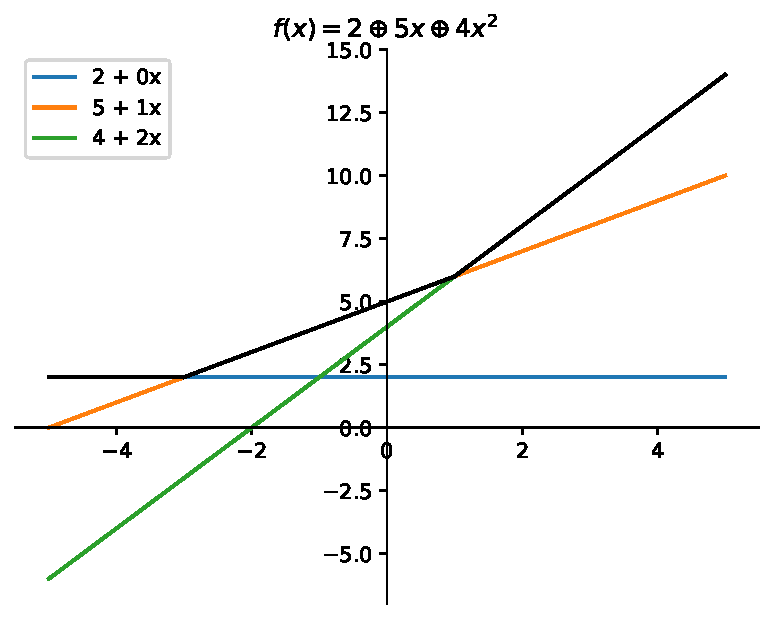
\includegraphics[scale=0.5]{graphics/first_trop_pol.pdf}
\subcaption{Take $f(x) = 2 \oplus 5x \oplus 4x^{2}$ a quadratic polynomial. The graph equals $max(2, 5+x, 4+2x)$. Until $5-2$, $2$ dominates, from there $5+x$ dominates to the point $4+2x$.}
\label{fig:trop_quad_1}
\end{subfigure}\hfill%
\begin{subfigure}[t]{0.48\textwidth}
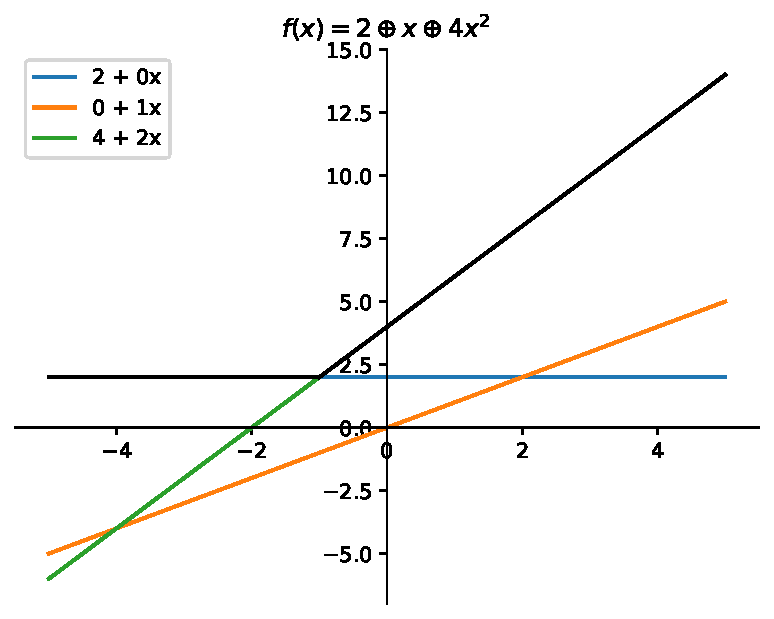
\includegraphics[scale=0.5]{graphics/second_trop_pol.pdf}
\subcaption{Take $f(x)=2 \oplus x \oplus 4x^{x}$, we have changed the scalar in the second part, then this second part plays no part in the tropical polynomial.}
\label{fig:trop_quad_2}
\end{subfigure}

\caption{Quadratic tropical polynomials.}
\label{fig:image2}
\end{figure}

We can see the degree of a tropical polynomial, defined the same as a degree of a usual polynomial, gives an upper bound for the number of non-linear edges of the tropical polynomial, but not the exact value. With higher degree polynomials more non linear edges are possible as figure \ref{fig:trop_qub} illustrates.


\begin{figure}[h]
\centering
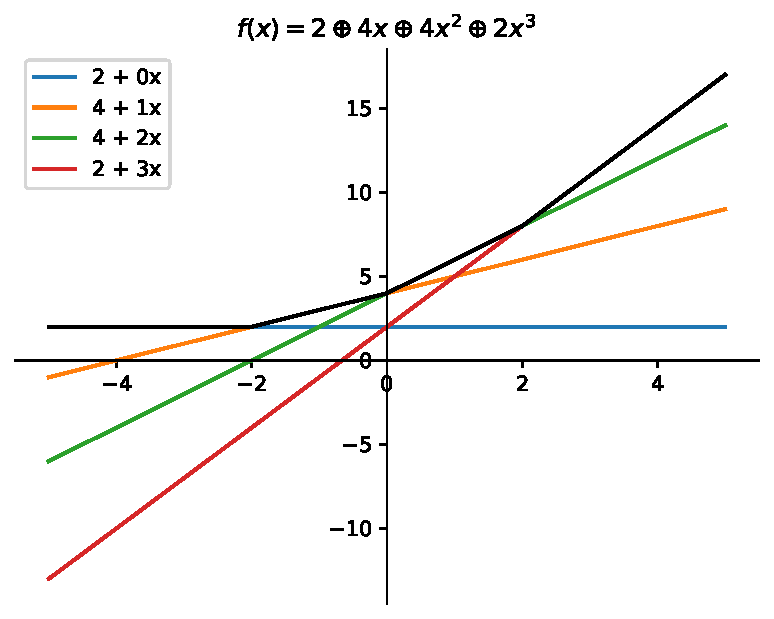
\includegraphics[scale=0.75]{graphics/third_trop_pol.pdf}
\caption{Take $f(x)=2 \oplus x \oplus 4x^{x} \oplus 4x^{2} \oplus 3x^{3}$. For a degree three tropical polynomial in one variable this polynomial has reached the maximum number of non linear edges.}
\label{fig:trop_qub}
\end{figure}
\end{remark}



\begin{definition}
Let $S$ be a set in a real vector space. Then $S$ is \textbf{convex} if for $s_{1}, s_{2} \in S$: 
$$\lambda s_{1} + (1-\lambda) S_{2} \in S$$
holds for all $\lambda \in [0,1] \subset \mathbb{R}$.
\end{definition}

\begin{definition}
Let $X$ be a convex set in a real vector space and let $f:X \to \mathbb{R}$ be a function, then $f$ is called \textbf{convex} if for $x_{1}, x_{2} \in X$ and $\lambda \in [0,1] \subset \mathbb{R}, f(\lambda x_{1} + (1-\lambda)x_{2}) \leq tf(x_{1}) + (1-t)f(x_{2})$ holds.
\end{definition}


\begin{definition}
A function $f : \mathbb{R}^{m} \to \mathbb{R}^{n}$ with $n, m \in \mathbb{N}$ is \textbf{piecewise linear} if there exist closed sets $(P_{i})_{i \in \mathbb{N}} \subset \mathbb{R}^{m}$ with $f : P_{i} \to K^{n}$ linear and $\cup_{i}P_{i} = K^{m}$.
\end{definition}

In multiple variables we can characterise tropical polynomials as functions from $\mathbb{R}^{n} \to \mathbb{R}$ that satisfy the following three properties.

\begin{lemma}\label{lemma:trop_properties}
Let f be a tropical polynomial
$$ f(x) = c_1 x^{\alpha_1} \oplus \dots \oplus c_r x^{\alpha_r}$$ as in definition \ref{def:tropPolyn}, but we restrict $c_1, \dots , c_r \in \mathbb{R}$ to be real and $f: \mathbb{R}^{n} \to \mathbb{R}$ with $n \in \mathbb{N}$. Then f has three important properties:
\begin{itemize}
\item[(1)]
$f$ is continuous.
\item[(2)]
$f$ is piecewise-linear, where the number of pieces is finite.
\item[(3)]
$f$ is convex, i.e. $p(\frac{x + y}{2}) \leq \frac{1}{2}(p(x)+p(y)) \forall x,y \in \mathbb{R}$
\end{itemize}
\end{lemma}

\begin{proof}
The minimum of continuous functions is still continuous which proves (1). Every monomial $c_ix^{\alpha_i} = c_i + x_{1}\alpha_{i1} + \dots + x_n \alpha_{in}$ is per definition linear. Because of (1), linearity can only be broken where $c_i x^{\alpha_i} = c_j x^{\alpha_j}$ for $i \leq j$ and $i,j = 1, \dots ,r$. A piece is a single maximal region of $c_ix^{\alpha_i}$ on which linearity is not broken. If we introduce $c_ix^{\alpha_i}$ one after another, then in the $i$-th step not more than $i^2$ new pieces can be created, so there can only be $ \sum_{i=1}^{r} i^2$ or less pieces which proves (2). 
For (3) let $x, y \in \mathbb{R}^{n}$, then:
\begin{align*}
f&(\lambda x + (1-\lambda)y) \\
&= \bigoplus^{r}_{i=1} c_{i}(\lambda x + (1-\lambda) y)^{\alpha_{i}} \\
&= \text{max}^{r}_{i=1} \{ c_{i} + \sum_{j=1}^{n} \alpha_{ij}(\lambda x_{j} + (1-\lambda) y_{j}) \} \\
&= \text{max}^{r}_{i=1} \{ \lambda (c_{i} + \sum_{j=1}^{n}\alpha_{ij}x_{j}) + (1-\lambda) (c_{i} + \sum_{j=1}^{n}\alpha_{ij} \ y_{j})\} \\
&\leq \text{max}^{r}_{i=1} \{ \lambda (c_{i} + \sum_{j=1}^{n}\alpha_{ij}x_{j}) \} + \text{max}^{r}_{i=1} \{ (1-\lambda) (c_{i} + \sum_{j=1}^{n}\alpha_{ij}y_{j}) \} \\
&= \lambda \ \text{max}^{r}_{i=1} \{ (c_{i} + \sum_{j=1}^{n}\alpha_{ij}x_{j}) \} + (1-\lambda) \ \text{max}^{r}_{i=1} \{ (c_{i} + \sum_{j=1}^{n}\alpha_{ij}y_{j}) \} \\
&= \lambda f(x) + (1-\lambda) f(y)
\end{align*}
which ends the prove.
\end{proof}

The same could be argued for our tropical function $f$, if we let $c_{i} \in \mathbb{T}$ and $f:\mathbb{T}^{n} \to \mathbb{T}$, but the underlying theories, for example for linearity, change for semifields\cite{olia2020analysis}.

\begin{proposition}
Every function $\mathbb{R}^{n} \to \mathbb{R}$ which satisfies the three properties (1), (2) and (3) from lemma 	\ref{lemma:trop_properties} has a representation as the minimum of a finite set of linear functions. Thus, the tropical polynomials in n variables $x_{1}, \dots x_{n}$ represent the class of piecewise-linear convex functions on $\mathbb{R}^{n}$ with integer coefficients.
\end{proposition}

\begin{proof}
This follows directly from lemma \ref{lemma:trop_properties}.
\end{proof}

Now we are ready to introduce tropical rational functions and the semifields $\mathbb{T}[X_{1} , \dots , X_{d}], \ \mathbb{T}(X_{1} , \dots , X_{d})$. These are important to understand the core section (section \ref{sec:trop_netw}), in particular the actual connection build between neural networks and tropical geometry in this thesis.

\begin{definition} \cite[p.~3]{zhang2018tropical}
A \textbf{tropical rational function} is a standard difference, or, equivalently, a tropical quotient of two tropical polynomials $f(x)$ and $g(x)$:
$$ (f-g)(x) = f(x) - g(x) = f(x) \oslash g(x) = (f \oslash g)(x)$$
%We will denote a tropical rational function by $f \oslash g$, where $f$ and $g$ are understood to be tropical polynomial functions.
\end{definition}
\begin{proposition}
\label{prop:trop_semi_ring_set}
The sets $\mathbb{T}[X_1, \dots , X_d] := \{ f: \mathbb{T}^{d} \to \mathbb{T} ; f \ \text{is tropical polynomial} \}$ and \ $ \mathbb{T}(X_1, \dots , X_d) := \{ f: \mathbb{T}^{d} \to \mathbb{T} ; f \ \text{is tropical rational function} \}$ are both semirings. \cite[p.~3]{zhang2018tropical}
\end{proposition}
\begin{proof}
We begin the proof by showing, that for two tropical polynomials $f, g \in \mathbb{T}[X_1, \dots , X_r]$ with $f(x) =\oplus_{i=0}^{\alpha} a_{i} x^{\zeta_{i}}$ and $g(x)= \oplus_{i=0}^{\beta} b_{i} x^{\omega_{i}}$ their tropical multiplication is a tropical polynomial $f \odot g \in \mathbb{T}[X_1, \dots , X_r]$.
\begin{align*} 
(f \odot g)(x) &= f(x) + g(x) \\
&=  (\bigoplus_{i=0}^{\alpha} a_{i} x^{\zeta_{i}}) + (\bigoplus_{i=0}^{\beta} b_{i} x^{\omega_{i}}) \\
&= \text{max}_{i=0}^{\alpha} \{ a_{i} + \sum_{k=1}^{r} \zeta_{ik} x_{k} \} + \text{max}_{j=0}^{\beta} \{ b_{j} + \sum_{k=1}^{r} \omega_{jk} x_{k} \} \\
&= \max_{\substack{
   i=1, \dots , \alpha \\
   j=1, \dots , \beta
  }} \{ a_{i} + \sum_{k=1}^{r} \zeta_{ik} x_{k} + b_{j} + \sum_{k=1}^{r} \omega_{jk} x_{k} \} \\
&= \max_{\substack{
   i=1, \dots , \alpha \\
   j=1, \dots , \beta
  }} \{ (a_{i} + b_{j} + \sum_{k=1}^{r} (\zeta_{ik} + \omega_{jk}) x_{k} \} \\
&= \bigoplus_{\substack{
   i=1, \dots , \alpha \\
   j=1, \dots , \beta
  }} \ (a_{i} \odot b_{j}) \odot x^{\zeta_{i} + \omega_{i}} \in \mathbb{T}[X_1, \dots X_r]
\end{align*}
That $(f \oplus g) \in \mathbb{T}[X_1, \dots X_r]$ is immediate. We have already shown that $\mathbb{T}$ is a tropical semifiled. Therefore, except for the neural elements, all other axioms hold automatically pointwise.

The neutral element for the tropical sum is $- \infty = - \infty \oslash x = x \oslash - \infty \ x \in \mathbb{T}$. Both $0, -\infty \in \mathbb{T}$ are also a tropical and tropical rational function. Since for $f(x) \in \mathbb{T}(X_1, \dots , X_r)$ or $f(x) \in \mathbb{T}[X_1, \dots , X_r]$, the following hold
\begin{align*}
&f(x) \oplus \infty = \max(f(x),\ - \infty) = f(x) \\
&f(x) \odot 0 = f(x) + 0 = f(x).
\end{align*} 
Therefore $0$ is the neutral element of tropical multiplication for tropical and tropical rations functions and $-\infty$ is the neural element of addition. We have shown $T[X_1, \dots X_r]$ is a semifield. \\ 
Let $g,f,h \in \mathbb{T}(X_1, \dots ,X_d)$ with 
\begin{align*}
f(x) &= f_1(x) \oslash f_2(x) \\
g(x) &= g_1(x) \oslash g_2(x) \\
h(x) &= h_1(x) \oslash h_2(x)
\end{align*}
The tropical sum of tropical rational functions is a tropical rational function:
\begin{align*}
(f \oplus g)(x) &= f(x) \oplus g(x) \\
&=(f_1(x) \oslash f_2(x)) \oplus (g_1(x) \oslash g_2(x)) \\
&= \min\{f_1(x) - f_2(x), g_1(x) - g_2(x) \} \\
&= \min\{f_1(x) + g_2(x), g_1(x) + f_2(x) \} - f_2(x) - g_2(x) \\
&= (f_1(x) + g_2(x) \oplus g_1(x) + f_2(x)) \\
& \ \ \ \ \oslash (f_2(x) + g_2(x)) \in \mathbb{T}(X_1, \dots , X_r).
\end{align*}
since addition as tropical addition of tropical polynomials is a tropical polynomial.
The tropical product of tropical rational functions is a tropical rational function:
\begin{align*}
(f \odot g)(x) &= f(x) \odot g(x) \\
&=  (f_1(x) \oslash f_2(x)) \odot (g_1(x) \oslash g_2(x)) \\
&= f_1(x) - f_2(x) + g_1(x) - g_2(x) \\
&= (f_1(x) + g_1(x)) - (f_2(x) + g_2(x)) \in \mathbb{T}(X_1, \dots , X_r)
\end{align*}
This concludes the proof.
\end{proof}

\begin{proposition}
The set $\mathbb{T}(X_1, \dots , X_d)$ is a semifiled.
\end{proposition}
\begin{proof}
Because of proposition \ref{prop:trop_semi_ring_set} we only have to show that $f \oslash g \in \mathbb{T}(X_1, \dots , X_d)$ has a multiplicative inverse element. With $(f \oslash g) \odot (g \oslash f) = f - g + g - f = 0$ we have found $(g \oslash f) \in \mathbb{T}(X_1, \dots , X_d)$ the element.
\end{proof}

We regard a tropical polynomial $f=f \oslash 0$ as a special case of a tropical rational function and thus $\mathbb{T}[X_1, \dots , X_r] \subseteq \mathbb{T}(X_1, \dots , X_r)$. \cite[p.~3]{zhang2018tropical}

\begin{remark}
% ~\
% \begin{itemize}
% \item[$\bullet$]
A d-variate tropical polynomial $f(x)$ defines a function $f: \mathbb{T}^{d} \to \mathbb{T}$ that is a convex function in the usual sense as taking $\max$ and $\sum$ of convex functions preserve convexity \cite{boyd2004convex}.
% \item[$\bullet$]
% As such, a tropical rational function $f \oslash g : \mathbb{T}^{d} \to \mathbb{T}$ is a DC function or differenceconvex function \cite{hartman1959functions}.
% \end{itemize}
\end{remark}

\begin{definition}
$R : \mathbb{R}^{d} \to \mathbb{R}^{p}, x = (x_1, \dots , x_d)\mapsto (f_1(x), \dots , f_p(x))$, is called a \textbf{tropical polynomial map} if each $f_i : \mathbb{R}^{d} \to \mathbb{R}$ is a tropical polynomial, $i = 1, \dots , p$, and a \textbf{tropical rational map} if $f_1, \dots , f_p$ are tropical rational functions. We will denote the set of tropical polynomial maps by $Pol(d, p)$ and the set of tropical rational maps by $Rat(d, p)$. So $Pol(d, 1) = \mathbb{T}[X_1, \dots , X_d]$ and $Rat(d, 1) = \mathbb{T}(X_1, \dots , X_d)$ \cite[p.~3]{zhang2018tropical}.
\end{definition}

Next we introduce deep neural networks.

\newpage

\section{Neural networks}
\label{sec:neural_networks}
Historically the term "Neural Network" was introduced in attempts to describe the functionality of biological processes, in particular the nervous system and the brain, in a mathematical sense \cite{mcculloch1943logical, widrow1960adaptive, rumelhart1986learning}. Simply put the nervous system is a net of neurons, each having a soma and an axon. "At any instant a neuron has some threshold, which excitation must exceed to initiate an impulse. This, except for the fact and the time of its occurrence, is determined by the neuron, not by the excitation. From the point of excitation the impulse is propagated to all parts of the neuron." \cite[p.~1]{mcculloch1943logical} Through synapses the axons are connected to the soma of further neurons, this way the impulse is passed on. Impulses passing through the nervous system partly consist of electrical impulses and chemical reactions \cite{palay1956synapses}. A collection of partially connected neurons, capable of carrying impulses, is called a biological neural network.


\begin{figure}[H]
\centering
\figuretitle{Depiction of a neuron}
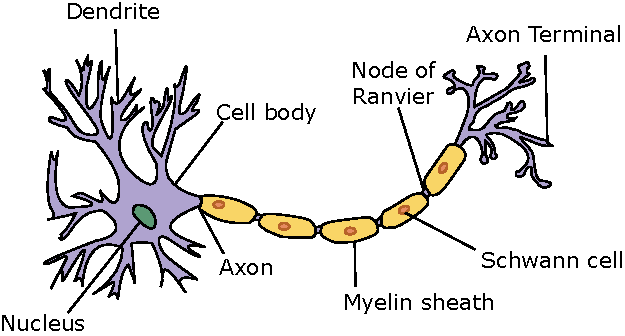
\includegraphics[scale=0.75]{graphics/neuron.pdf}
\caption{A representation of a neuron. The axon terminal attach to dendrite. This way impulses pass from neuron to neuron\cite{neuron2020}.}
\label{fig:neuron}
\end{figure}

Based on a biological neural network, an abstract neuronal network, in the following simply referenced as neural network, is defined. Biological neurons and especially biological neural networks are far more complex than this introduction may make it seem. Because of their vast complexity biological realism would impose entirely unnecessary constraint when building a fast computable model. Boiling a biological neuronal network down to its quintessential features results in a weighted directed graph, where edges and vertices are weighted. Typically a weighted graph only has its edges weighted. To fit our model we introduce them also with weighted vertices.

\begin{definition}\cite[p.~148]{bender2010lists}
A \textbf{finite graph} or simply \textbf{graph} is a pair $G = (V, E)$, where $V$ is a finite set whose elements are called vertices, and $E \subset \{ \{x, y\}|(x,y) \in v^{2} \}$ is a set of two-sets of vertices, whose elements are called edges.
\end{definition}

A small tweak to this definition yields the definition of a directed graph.

\begin{definition}
A \textbf{directed graph} is a pair $G = (V, E)$, where $V$ is a set whose elements are called vertices, and $E \subset \{ (x, y)|(x,y) \in v^{2} \}$ is a set of edges which are ordered pairs of distinct vertices.
\end{definition}

\begin{definition}
Let $\mathbb{K}$ be a filed. A \textbf{vertex weighted graph} $G = (V, E, \psi)$ is a graph with a functions $\psi : V \to \mathbb{K}$ that assign a weight $\psi(v)$ to each vertex $v \in V$ and an \textbf{edge weighted graph} $G = (V, E, \omega)$ is a graph $G$ with a function $\omega : E \to \mathbb{K}$ that assigns a weight $\omega(e)$ to each edge $e \in E$. \\
A \textbf{weighted graph} $G = (V, E, \psi, \omega)$ or short $G = (V, E)$ is a graph with weighted edges and vertices.
\end{definition}

%\begin{definition}
%Let $G = (V, E)$ be a Graph. We set $n(G) = |V|$ to be the cardinality of vertices and $m(G) = |E|$ the cardinality of edges.
%\end{definition}

Graphs can represent a multitude of relations between objects. Like road maps of roads connecting cities. Or describe objects themselves like molecules.

\begin{example}
For instance the edge weighted directed Graph $G = (V, E, \omega)$ depicted in figure \ref{fig:mindDistGraph} could depict a map of hiking trails with connect huts as nodes. The trails are weighted with the distance between huts and we want to find the minimal walking distance from hut A to any other.\
We will use the opportunity to introduce a specific graph formally. Matching figure \ref{fig:mindDistGraph} the graph is fully defined by setting $V=\{\text{A}, \text{B}, \text{C}, \text{D}, \text{E}, \text{F}, \text{G}, \text{H}\}$, $E=\{(\text{A}, \text{B}), (\text{A}, \text{H}), (\text{A}, \text{E}), (\text{B}, \text{D}), \\ (\text{B}, \text{C}), (\text{B}, \text{H}), (\text{C}, \text{D}), (\text{C}, \text{G}), (\text{D}, \text{G}), (\text{E}, \text{H}), (\text{E}, \text{F}), (\text{E}, \text{G}), (\text{F}, \text{C}), (\text{F}, \text{G}), (\text{H}, \text{C}), \\ (\text{H}, \text{F})\}$ and in the same order as we have written the edges of $E$ here, the values of $\omega$ correspond to $5, 8, 9, 15, 12, 4, 3, 11, 9, 5, 4, 20, 1, 13, 7, 6$.

\begin{figure}[H]
\centering
\figuretitle{Min distance weighted graph}
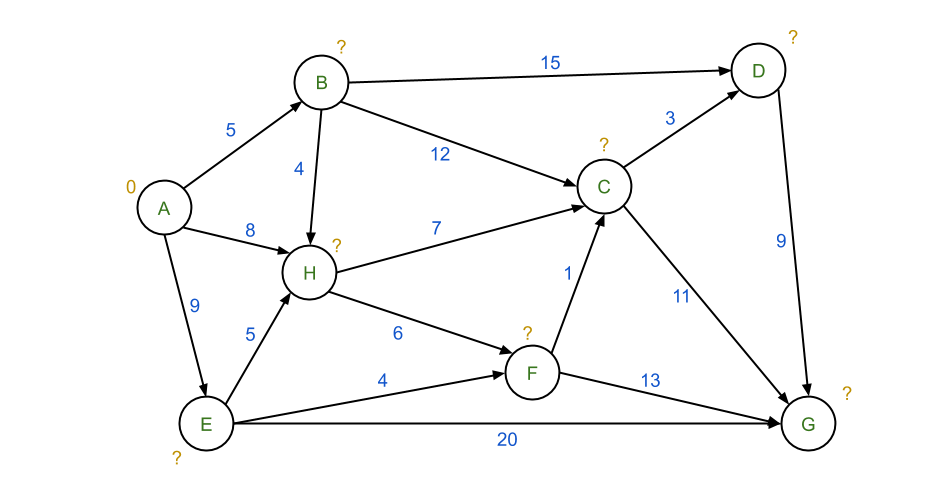
\includegraphics[scale=0.8]{graphics/weighted_directed_graph_2.png}
\caption{Min distance weighted graph \cite{dijacGraph20}.}
\label{fig:mindDistGraph}
\end{figure}

To compute an answer we use Dijkstra's algorithm. At any point in the algorithm simply consider all reachable nodes from nodes that have their shortest path already computed by adding up the computed shortest paths length to the paths length to the reachable node. This way every reachable node by nodes with there longest path already computed get at least one or multiple lengths of paths assigned to them. Pick the shortest path under all of these and repeat until all vertices have a path assigned. If there are multiple shortest paths, pick one of them. At any point, if there are no more reachable nodes, terminate and the nodes that have no distance assigned are not reachable.
\begin{proof}
Let $v_0 \in V$ be our starting vertex and $v_1$ an adjacent vertex with the closest path to $v_0$. Say $\text{dist}(v)$ is the computed shortest distance from node $v_0$ to $v \in V$, then $\text{dist}(v_1) = \omega((v_0, v_1))$. Let $n \in \mathbb{N}$, now say $v_1, \dots , v_n$ are the $n$ nodes with the shortest paths $\text{dist}(v_1), \dots , \text{dist}(v_n)$ and $v_{n+1} \in V \setminus {v_1, \dots , v_n}$ the vertex of closest distance to one of $v_1 \dots v_n$ out of all adjacent vertices. We pick $i \in \{ 1 , \dots , n \}$ so that $v_i$ is the vertex to which $v_{n+1}$ is closest, then $\text{dist}((v_1, v_{n+1}))$ since otherwise $v_{n+1}$ would have been under the first $n$ closest vertices. Also $v_1 , \dots , v_{n+1}$ are the $n+1$  closest vertices to $v_0$
\end{proof}

This way it is easy to compute, that the shortest distance to from node A to D is $17$ for example. \\
An interesting link to tropical geometry in this example is, if we write the edges of a graph as a matrix in the following form
$$M := \left[ \begin{array}{rrrr}
(v_0, v_0) & (v_0, v_1) & \cdots \\
(v_1, v_0) & (v_1, v_1)  \\
\vdots &  & \ddots \\
\end{array}\right]$$
then $(M^{k})_{ij}$ returns the shortest distance from $v_i$ to $v_j$ after $k$ steps.
\end{example}

Graph theory is a big field, but we are interested in modelling neural networks. In particular in those neural networks that have specific input layers and output layers. Our goal at this point is to get an insight of how to construct a neural network and define weights, so that our output stands in a predefined relation to our input.
In particular one of the most important neural networks is the L-layer feedforward neural network. \
We will define and motivate L-layer feedforward neural networks using graphs at first and then abstract again to only their necessary features.

\begin{definition}
\label{def:graphFeedForwardNetwork}
An \textbf{L-layer feedforward neural network} in graph form $(G, \sigma)$ is a weighted graph $G=(V, E)$ with a piecewise differentiable activation function $\sigma: \mathbb{R} \to \mathbb{R}$. The graph consists of $L$ sets $V^{(j)}$, $j = 1, \dots , L$ of vertices $V=\cup_{j=1}^{L}V^{(j)}$ with $L-1$ corresponding sets of edges $E^{(i)} \subset \{(x,y)|x \in V^{(i)}; y \in V^{(i+1)}\}$, $i = 1, \dots , L-1$ and $E=\cup_{i=1}^{L-1}E^{(i)}$ which connect two consecutive layers.
\end{definition}

The Graph of a $0$-layer feedforward neural network is an empty graph and of a $1$-layer feedforward neural network is a set of vertices without connecting edges. The \textbf{activation function} $\sigma$ will be applied in between propagating nodes in forward propagation \ref{def:forward_propagation}.

\begin{definition}
The first layer of an $L$-layer feedforward neural network is called the \textbf{input layer} and the last ($L$-th) layer is called the \textbf{output layer}. All layers in between collectively are called \textbf{hidden layers}.
\end{definition}

\begin{definition}
A $L$-layer feedforward neural network $(G, \sigma)$ with $G = (V, E)$ is called \textbf{fully connected} if $E$ is the largest out of every possible sets of $E$.
\end{definition}

In a fully connected feedforward neural network every vertex of $V^{(j)}$ is connected though an edge to a vertex of $V^{(j+1)}$ for each $j = 1, \dots , L-1$.

\begin{example}
We will construct a simple fully connected 4-layer feedforward neural network for the sake of visualisation. Using the same notation as in definition \ref{def:graphFeedForwardNetwork} we set $V^{(1)}=\{v_{11}, v_{12}, v_{13}, v_{14}\}, V^{(2)}=\{v_{21}, v_{22}, v_{23}\}, V^{(3)}=\{v_{31}, v_{32}, v_{33}\}$ and $V^{(4)}=\{v_{41}\}$. The edges are immediately defined when the vertices are defined in a fully connected graph. For example $E^{(3)}=\{(v_{31}, v_{41}), (v_{32}, v_{41}), (v_{33}, v_{41})\}$ is forced. As the use of weights is not introduced jet we set them all to $1$ for example and draw the graph in figure \ref{fig:4LayerNetwork}: 
\begin{figure}[H]
\centering
\figuretitle{Fully connected 4-layer feedforward neural network}
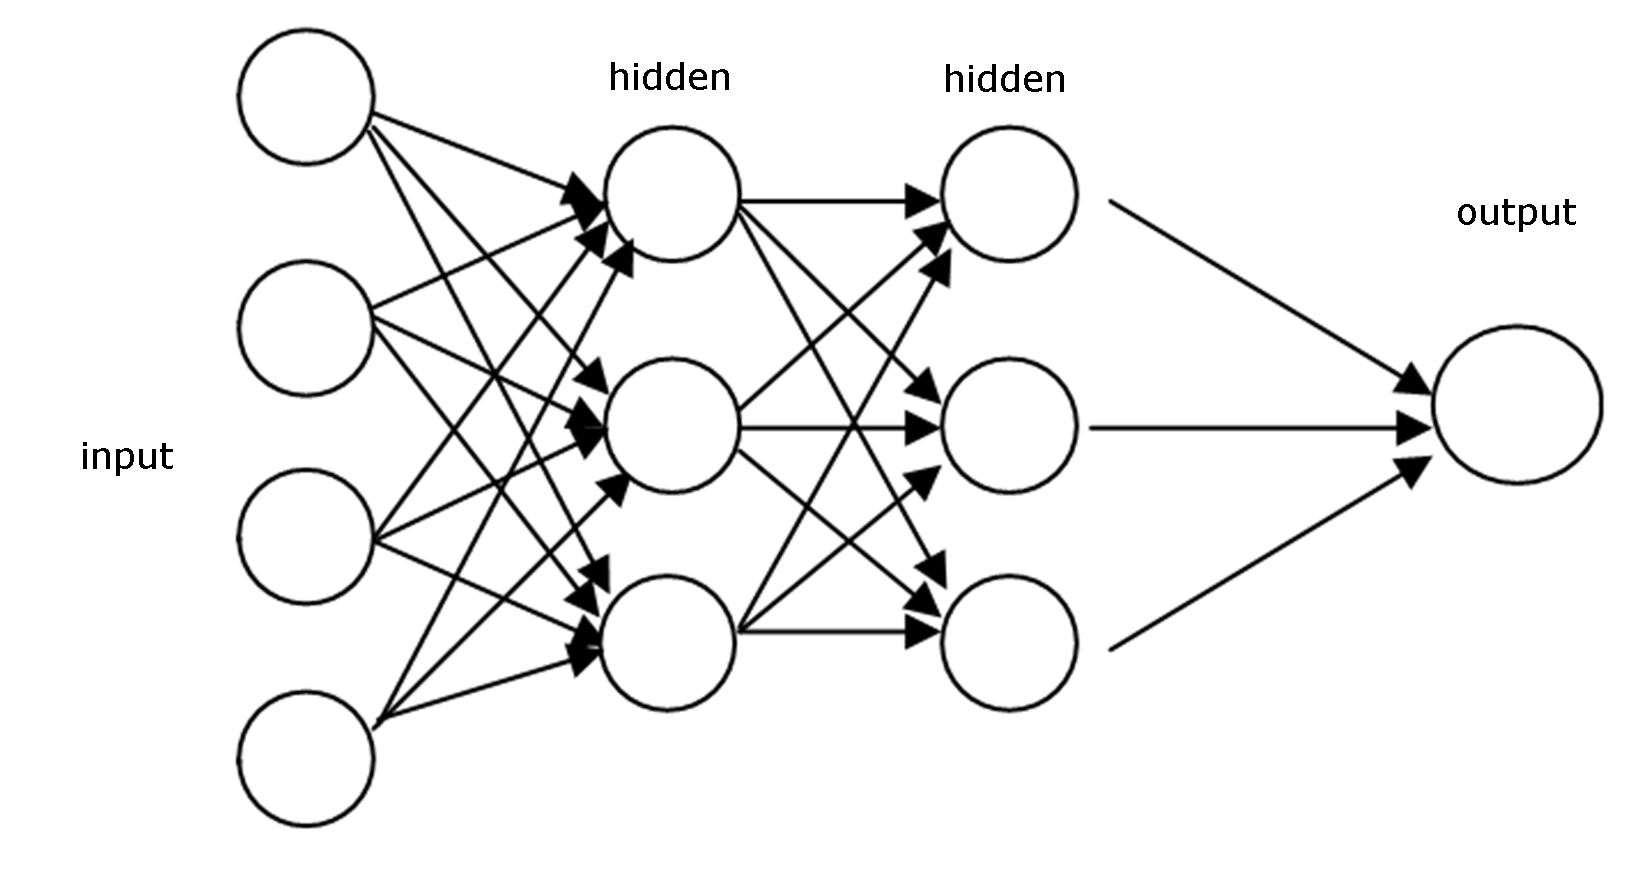
\includegraphics[scale=0.85]{graphics/MultiLayerNeuralNetwork.png}
\caption{An example image of a fully connected feedforward neural network without visualised edge and vertex weights\cite{neuralNetwork2020}.} 
\label{fig:4LayerNetwork}
\end{figure}

\end{example}

Inspired by biological neural networks, which are the core building blocks of animal brains, we have abstracted some of the essential features, given an introduction to graphs and used these as a mathematical buildingblock for neural networks.
With the introduction of feedforward neural networks we have cast a sensible form of neural network with which we will be able to store and also learn complex relations between input data and output data through forward and backward propagation. These will be introduced now.\\
Forward propagation describes the process by which from an input vector the output vector is calculated. First we need to introduce the bias vectors and weight matrices.

\begin{remark}\label{standardGraphLabeling}
Let $(G, \sigma)$ be a $L$-layer feedforward neural network, with $G=(V,E,\psi,\omega)$, where we name the elements from the sets $V^{(j)} = \{ b_{j1}, \dots ,b_{j|V^{(j)}|} \}$ so that these are ordered. The \textbf{bias vector} of layer j: 
$$b^{(j)} = (\psi(b_{j1}), \dots ,\psi(b_{j|V^{(j)}|}))^{t},$$ 
corresponds to the weights of vertices in $V^{(j)}$ for $j = 2, \dots , L$. The \textbf{weights matrix} $W^{(j)}$ with the entries 
$$W^{(j)}_{nm} = \omega((b_{j-1n}, b_{jm}))$$ 
corresponds to the matrix of weights of edges connecting layer $j-1$ and $j$ where $j$ is still in range $j = 2, \dots , L$.
\end{remark}

We will label feedforward neural networks this way until we define feedforward neural networks as functions and are now in a position to define forward propagation.

\begin{definition}(Forward Propagation)
\label{def:forward_propagation}
Let $(G, \sigma)$ be as in \ref{standardGraphLabeling} a $L$-layer feedforward neural network. Let $a^{(1)} = x \in \mathbb{R}^{|V^{(1)}|}$ be the input vector of the same dimension as the cardinality of the first layer $V^{(1)}$ of the neural network, then recursively we define $z^{(j)} = W^{(j)} a^{(j-1)} + b^{(j)}$ and $a^{(j)} = \sigma(z^{(j)})$, for $j=2, \dots , L$. A \textbf{forward propagation} of our $L$-layer feedforward neural network $(G, \sigma)$ is defined to be the value of $a^{(L)}$.
\end{definition}

For the sake of proving that the feedforward neural networks we have defined are able to be set up, so that for any specific binary input any binary specific output can be obtained, we will view the infrastructure of the weights, bias and the function $\sigma$ together as a circuit. Often binary inputs, as for example black and
\begin{wrapfigure}{r}{0.68\textwidth}
\centering
%\figuretitle{Min distance weighted graph}
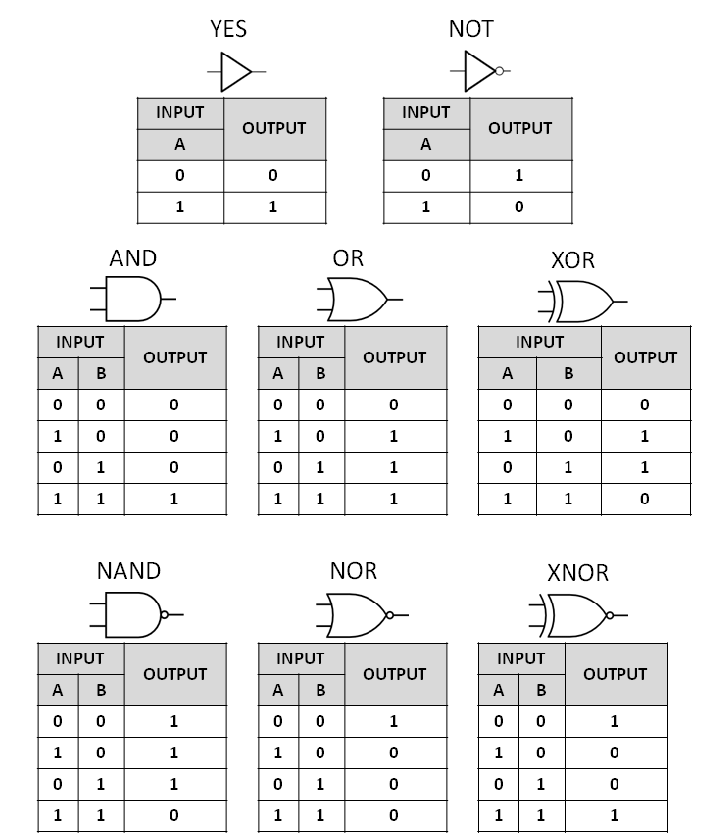
\includegraphics[scale=0.2]{graphics/Summary-of-the-common-Boolean-logic-gates-with-symbols-and-truth-tables.png}
\caption{Boolean Gates Truth Tables \cite{booleanGates}}
\label{fig:bool_gate}
\end{wrapfigure}
white pictures, are fed into neural networks and binary outputs, like dogs or cats are expected.

\begin{remark}
Binary circuits are defined by basic logical gates like AND, OR, and NOT gates and a lot more, that manipulate binary input as shown in figure \ref{fig:bool_gate}. A set of gates is called a \textbf{Universal Logic Gates Set} if with those gates any other logic or boolean function can be created. After \cite{quine1955way} AND, OR and NOT define such a set. Thsi meanings, if we can reproduce these three gates in form of feedforward neural networks, any boolean logic can be created by these. For that we set $\omega=\mathds{1}$, the weights of edges to one and
\[ \sigma(x) = 
  \begin{cases}
    1       & \quad \text{if } x > 0\\
    0  		& \quad \text{if } x \leq 0.
  \end{cases}
\]
%Then again NAND and NOR both can make a AND, OR and NOT gait, so ether of them are so called minimal universal logic gates, meaning they can make any other logic of Boolean function on their own.
Usually the output of a neural network is non binary, but is trained so that the higher the output value is the higher the probabillity of the specific outcome and the lower the output the lower the probability, with zero being neutral. To fit this interpretation $\sigma$ is defined to immediately produce a binary output. Now we will define three different $2$-layer feedforward neural nets with this sigma.


\begin{figure}[H]
    \centering
    \begin{subfigure}[b]{0.3\textwidth}
    	\centering
        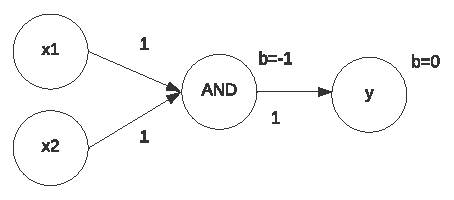
\includegraphics[width=\textwidth]{graphics/AND_gate.pdf}
        \caption{AND gate}
        \label{fig:AND}
    \end{subfigure}
    \begin{subfigure}[b]{0.3\textwidth}
    	\centering
        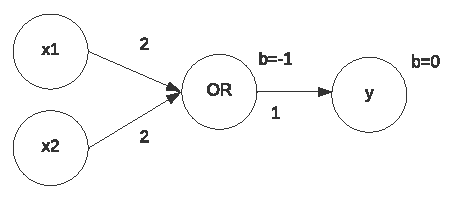
\includegraphics[width=\textwidth]{graphics/OR_gate.pdf}
        \caption{OR gate}
        \label{fig:OR}
    \end{subfigure}
    \begin{subfigure}[b]{0.3\textwidth}
    	\centering
        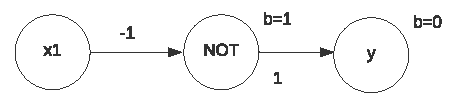
\includegraphics[width=\textwidth]{graphics/NOT_gate.pdf}
        \caption{NOT gate}
        \label{fig:NOT}
    \end{subfigure}
    \caption{Neural Logical Gates}\label{fig:neural_logic_gates}
\end{figure}
Each network takes a real vector $x$ as input and returns $y$. The weights of each layer are attached to the edges and the biases are labelled with "b". The first gate, shown in figure \ref{fig:neural_logic_gates} (a), defines our AND gate. It is defined with the graph $G=(E, V)$, $V=\{ b_{11}, b_{12}, b_{21}, b_{31} \}$, $E=\{ (b_{11}, b_{21}), (b_{12}, b_{21}), (b_{21}, b_{31})\}$ a fully connected neural network with weights 
$$\psi(b_{11})=\psi(b_{12})=\psi(b_{31})=0, \ \psi(b_{21})=-1 \ and \ W^{(1)}=\begin{pmatrix}1\\1\end{pmatrix}, \ W^{(2)}=\begin{pmatrix}1\end{pmatrix}.$$
The first index of every bias corresponds to the layer. Lets compare the the boolean output with the truth table. Inputs $\{(x, y)|x, y \in \{0, 1\}\}$ with
$$z^{(1)}=(1, 1)\begin{pmatrix}x\\y\end{pmatrix}-1 \ \to \ z^{(2)} = (1)(\sigma(x+y-1))+0 = \sigma(x+y-1)$$
\begin{align*}
\text{for} \ (0, 0) \ \text{yield} \ z^{(2)}&=\sigma(-1)=0 \\
\text{for} \ (1, 0), (0, 1) \ \text{yield} \ z^{(2)}&=\sigma(0)=0 \\
\text{and} \ for \ (1, 1) \ \text{yield} \ z^{(2)}&=\sigma(1)=1.
\end{align*}
The same graph with weights
$$\psi(b_{11})=\psi(b_{12})=\psi(b_{31})=0, \ \psi(b_{21})=-1 \ and \ W^{(1)}=\begin{pmatrix}2\\2\end{pmatrix}, \ W^{(2)}=\begin{pmatrix}1\end{pmatrix}$$
makes an OR gate:
$$z^{(1)}=(2, 2)\begin{pmatrix}x\\y\end{pmatrix}-1 \ \to \ z^{(2)} = (1)(\sigma(2x+2y-1))+0 = \sigma(2x+2y-1)$$
\begin{align*}
for \ (0, 0) \ yield \ z^{(2)}&=\sigma(-1)=0 \\
for \ (1, 0), (0, 1) \ yield \ z^{(2)}&=\sigma(2)=1 \\
and \ for \ (1, 1) \ yield \ z^{(2)}&=\sigma(4)=1.
\end{align*}
And last but not least the graph of the NOT gate is different in that it only has one input. Therefore the graph also changes to $G=(E, V)$, $V=\{ b_{11}, b_{21}, b_{31} \}$, $E=\{ (b_{11}, b_{21}), (b_{21}, b_{31})\}$ also a fully connected $2$ feedforward neural network. With weights
$$\psi(b_{11})=\psi(b_{31})=0, \ \psi(b_{21})=1 \ and \ W^{(1)}=(-1), \ W^{(2)}=(1)$$
that define a NOT gate:
\begin{align*}
for \ (0) \ yield \ z^{(2)}&= z^{(1)} = 1 \\
and \ for \ (1) \ yield \ z^{(2)}&= z^{(1)} = 0.
\end{align*}

We have proven that any binary input can create any binary output. This also means that by scaling the input and output weights it is possible from any specific input to create any specific output.

\end{remark}

The last abstraction level of feedforward neural networks is to define them as a function, which enables to us to compare feedforward neural networks to tropical polynomials in Chapter $4$.

\begin{definition}\cite{zhang2018tropical}
Viewed abstractly, an \textbf{L-layer feedforward neural network} is a map $\nu : \mathbb{R}^{d} \to \mathbb{R}^{p}$ given by a composition of functions
$$ \nu = \sigma^{(L)} \circ \rho^{(L)} \circ \sigma^{(L-1)} \circ \rho^{(L-1)} \circ \dots \circ \sigma^{(1)} \circ \rho^{(1)}$$
The preactivation functions $\rho^{(1)}, \dots , \rho^{(L)}$ are affine transformations to be determined and the activation functions $\sigma^{(1)}, \dots , \sigma^{(L)}$ are chosen and fixed in advanced. \\
We denote the width, i.e., the number of nodes, of the $l$-th
layer by $n_l, l = 1, \dots , L-1$. We set $n_0 := d$ and $n_L := p$, respectively the dimensions of the input and output of the network. The output from the $l$-th layer will be denoted by
$$\nu^{(l)} = \sigma^{(l)} \circ \rho^{(l)} \circ \sigma^{(l-1)} \circ \rho^{(l-1)} \circ \dots \circ \sigma^{(1)} \circ \rho^{(1)}$$
i.e., it is a map $\nu^{(l)} : \mathbb{R}^{d} \to \mathbb{R}^{n_l}$. For convenience, we assume $\nu^{(0)}(x) := x$. \\
The affine function $\nu^{(l)} : \mathbb{R}^{n_{l-1}} \to \mathbb{R}^{n_{l}}$ is given by a weight matrix $A^{(l)} \in \mathbb{Z}^{n_l \times n_{l-1}} $ and a bias vector $b^{(l)} \in \mathbb{R}^{n_l}$:
$$ \rho^{(l)}(\nu^{(l-1)}) := A^{(l)} \nu{(l-1)} + b^{(l)}. $$
The $(i, j)$th coordinate of $A^{(l)}$ will be denoted $a^{l}_{ij}$ and the $i$th coordinate of $b^{(l)}$ by $b^{(l)}_{i}$. Collectively they form the parameters of the $l$th layer
\end{definition}

This way forward propagation corresponds to evaluation of the neural network.

\begin{remark}\cite{zhang2018tropical}
For a vector input $x \in \mathbb{R}^{n_l}, \sigma^{(l)}(x)$ is understood to be in coordinatewise sense; so $\sigma : \mathbb{R}^{n_l} \to \mathbb{R}^{n_l}$.
\end{remark}
\begin{remark}\cite{zhang2018tropical}
\label{rem:score_fkt}
We assume the final output of a neural network $\nu(x)$ is fed into a \textbf{score function} $s : \mathbb{R}^{p} \to \mathbb{R}^{m}$ that is application specific. The score function is quite often regarded as the last layer of a neural network but this is purely a matter of convenience and we will not assume this.
\end{remark}

Now we will give a brief introduction to backpropagation of neural networks. The underlying analytics for the small section of backpropagation will not be carried out in detail, rather they will be required as prerequisite knowledge from the reader. \
Backpropagation is best explained by viewing a feedforward neural network as a function or a concatenation of functions, which we can extend to a Cost function and perform gradient descent on.
In the following we may refer to $A^{(l)}$ as $w^{(l)}$ the \textbf{weight matrices} and $b^{(l)}$ simply as the \textbf{bias vectors}.

\begin{remark}
For a multi-variate function $F(X)$ that is defined and differentiable in a neighbourhood of a point $a$, then $F$ increases in point $a$ fastest in value in the direction of the gradient $\text{grad}(F)(a)$.
\end{remark}\label{rem:gradient}
This motivates the following definition.

\begin{definition}(Gradient descent)
It follows from remark \ref{rem:gradient} that for a differentiable function $F: \mathbb{R} \to \mathbb{R}$, if 
$$a_{n+1}=a_{n}-\epsilon \cdot \text{grad}(F)(a_{n})$$
for $\epsilon \in \mathbb{R}_{+}$ small enough and $a_{n} \in \mathbb{R}$, that $F(a_{n}) \geq F(a_{n+1})$. With this observation in mind, one starts with a guess $x_{0} \in \mathbb{R}$ for a local minimum of $F$, defines the sequence $(x_{n})_{n\in\mathbb{N}}$ as above ($c_{n+1}=c_{n}-\epsilon \cdot \text{grad}(F)(x_{n})$) and with epsilon small enough $x_{n}$ will eventually end up close to a local minimum. Setting up and calculating the sequence $x_{n}$ to step towards local minima is called gradient descent.
\end{definition}

We will use gradient descent with a cost function that we want to optimize the neural network on. To optimize a feedforward neural network to give sensible outputs relative to the inputs, we define the cost function.

\begin{definition}(Cost function)
\label{def:cost_fct}
Let $\nu : \mathbb{R}^{d} \to \mathbb{R}^{p}$ be a $L$-layer feedforward neural network and $s : \mathbb{R}^{p} \to \mathbb{R}^{m}$ a score function. The cost function for $\nu$ to a specific input $x$ and desired output $y$ is $C_{x}$ or $C_{x}(s(\nu(x)), y)$ being a differentiable extension of $\nu$ dependant on the weights and biases of $\nu$. We will assume the score function is considered in the definition of the cost function and simply write $C_{x}(\nu(x), y)$ instead. Notice that the input-output pair $(x, y)$ is fixed, where the weights $w^{(l)}$ and biases $b^{(l)}$ are variable. \\
The cost function of a finite set $\mathcal{X}$ of input vectors is then the average $$C=\frac{1}{|\mathcal{X}|}\sum_{x \in \mathcal{X}}C_{x}$$
over cost functions $C_{x}$ for individual training examples, x.
\end{definition}

%\begin{remark}
%The cost function is meant to be defined in relation to the score function to ensure, that lower values in the score function correspond to 
%\end{remark}

Backpropagation is an algorithm to tweak weights of a neural network to minimize the cost function on a training set, containing input vectors and the corresponding desired outputs. For our theoretical analysis of backpropagation we limit ourselves to the case where the $\sigma$ of feedforward neural networks are all differentiable. For a discussion of the general case of piecewise linear activation functions, we refer the reader to \cite{agostinelli2014learning}.

\begin{definition}(Backpropagation)
Let $\nu$ be an $L$-layer feedwordward neural network, $\mu \in \mathbb{R}$ a learning rate and $C$ be a cost function over $\nu$ as in \ref{def:cost_fct}. Application of backpropagation to $\nu$ is calculating $\text{grad}_{w^{(i)}}(C)$ the gradient of the weights and $\text{grad}_{b^{(i)}}(C)$ the gradient of the biases of the cost function for $i = 1, \dots , L$ and applying changes to the weights and biases of the neural network $\nu$ as follows:
\begin{align*}
w^{(i)} &\to (w^{(i)})' = w^{(i)}-\mu \cdot \text{grad}_{w^{(i)}}(C) \\
b^{(i)} &\to (b^{(i)})' = b^{(i)}-\mu \cdot \text{grad}_{b^{(i)}}(C) \ \text{for} \ i = 1, \dots, L.
\end{align*}
\end{definition}

Repeated application of backpropagation is a gradient descent algorithm and therefore optimizes the cost function and approaches local minima. This gives a way to train a neural network on a datapool efficiently.

\begin{remark}
\label{com:back_prop_madness}
Essentially, backpropagation evaluates the expression for the derivative of the cost function as a product of derivatives between each layer from left to right – "backwards" – with the gradient of $\sigma$'s between each layer being a simple modification of the partial products (the "backwards propagated error").
Given an input–output pair $(x,y)$, the loss is:
$$C_{x}(\sigma^{(L)} \circ \rho^{(L)} \circ \sigma^{(L-1)} \circ \rho^{(L-1)} \circ \dots \circ \sigma^{(1)} \circ \rho^{(1)}(x), y).$$


The gradient $\text{grad}$ is the transpose of the derivative of the output in terms of the input.

To understand how the algorithm of gradient descet operates, we first interpret the constant $x$ as a variable and $b^{(l)}, w^{(l)}$ as constants again. Then with the chain rule the following holds:
\begin{align*}
\frac{\mathrm \partial C_{x}}{\mathrm \partial x} &= \frac{\mathrm \partial C_{x}}{\mathrm \partial \sigma^{(L)}} \cdot \frac{\mathrm \partial \sigma^{(L)}}{\mathrm \partial \rho^{(L)}} \cdot \frac{\partial \rho^{(L)}}{\partial \sigma^{(L-1)}} \cdot \ \ldots \ \cdot \frac{d \sigma^{(1)}}{\partial \rho^{(1)}} \cdot \frac{\partial \rho^{(1)}}{\partial x}\\
 &= C_{x}'(\overline{\sigma^{(L)}}(x)) \cdot (\sigma^{(L)})'(\overline{\rho^{(L)}}(x)) \cdot \dots \cdot (\sigma^{(1)})'(\overline{\rho^{(1)}}(x)) \cdot (\rho^{(1)})'(x) \\
\text{grad}_{x} (C_{x}) &= \left(\frac{\partial C}{\partial x}\right)^{t}.
\end{align*}
Here sigma and rho bar are defined as follows:
\begin{align*}
\overline{\sigma^{(l)}} &= \sigma^{(l)} \circ \rho^{(l)} \circ \dots \circ \sigma^{(1)} \circ \rho^{(1)} \\
\overline{\rho^{(l)}} &= \rho^{(l)} \circ \sigma^{(l-1)} \circ \dots \circ \sigma^{(1)} \circ \rho^{(1)}.
\end{align*}
The affine linear functions $\rho^{(l)}$ for $l=L, \dots , 1$ can be written unambiguously as it's weight matrix $w^{(l)}$ and bias vector $b^{(l)}, \rho^{(l)} = x^{(l)} x + b^{(l)}$. 
With this form in mind we set $x$ constant again and in the $l$-th step view $w^{(l)}$ and $b^{(l)}$ as variable again. Then

\begin{align*}
\delta^{(L)} &= \frac{\partial C}{\partial \sigma^{(L)}} \cdot \frac{\partial \sigma^{(L)}}{\partial \rho^{(L)}} \\
\delta^{(l-1)} &= \delta^{(l)} \frac{\partial \rho^{(l)}}{\partial \sigma^{(l-1)}} \cdot \frac{\partial \sigma^{(l-1)}}{\partial \rho^{(l-1)}}, \\
\end{align*}
for $l=L-1, \dots, 1$.
This, depending on the choice of sigma, gives an easy to calculate algorithm for the gradients:
\begin{align*}
\grad_{w^{(l)}}(C_x) &= \left[\delta^{(l)} \cdot \frac{\partial \rho^{(l)}}{\partial w^{(l)}}\right]^{T} \\
\grad_{b^{(l)}}(C_x) &= \left[\delta^{(l)} \cdot \frac{\partial \rho^{(l)}}{\partial b^{(l)}}\right]^{T}.
\end{align*}
This is much faster than calculating the deltas in a forward manner with would have the following form:
\begin{align*}
\delta^{(1)} &= \frac{\mathrm \partial C_{x}}{\mathrm \partial \sigma^{(L)}} \cdot \frac{\mathrm \partial \sigma^{(L)}}{\mathrm \partial \rho^{(L)}} \cdot \frac{\partial \rho^{(L)}}{\partial \sigma^{(L-1)}} \cdot \ \ldots \ \cdot \frac{d \sigma^{(1)}}{\partial \rho^{(1)}} \\
&\vdots \\
\delta^{(L)}_{w} &= \frac{\partial C}{\partial \sigma^{(L)}} \cdot \frac{\partial \sigma^{(L)}}{\partial \rho^{(L)}}.
\end{align*}
The recursive way of propagating the neural network backwards is where backpropagation gets its name from. The $\overline{\sigma^{(l)}}$ and $\overline{\rho^{(l)}}$ for $l = 1, \dots , L$ get computed and saved beforehand in a forward propagation run to save computational time.

Now if we have a training set $\mathcal{X}$ of input and desired output pairs. What we want to compute is
\begin{align*}
\grad_{w^{(l)}}(C) &= \frac{1}{|\mathcal{X}|}\sum_{x \in \mathcal{X}}\grad_{w^{(l)}}(C_x) \\
\grad_{b^{(l)}}(C) &= \frac{1}{|\mathcal{X}|}\sum_{x \in \mathcal{X}}\grad_{b^{(l)}}(C_x)
\end{align*}
the gradients corresponding to the set. Because gradient decent is biased on iterative application, usually $\mathcal{X}$ is split up in $batches$, these are subsets of $\mathcal{X}$ of a set cardinality. This way the weights and biases get optimized on the batches itteratively. This method gets especially effective on large datapools $\mathcal{X}$.
\end{remark}


%\begin{remark}
%With a neural network as in \ref{com:back_prop_madness}, setting $\sigma^{(l)} = id$ and $\rho^{(l)} = w^{(l)} x$ a linear function for a weight matrix $w^{(l)}$. The Gradient derivative
%$fraq$
%\end{remark}

This gives a way to train neural networks on a datapool. There are a number of further topics to understand state of the art training of neural networks, for example stochastic gradient descent or over fitting. In this thesis, when it comes to training a neural network, the goal was to give only a basic overview. The main subject of this thesis is tropical algebra of neural networks.
\newpage

\section{Tropical algebra of neural networks}\label{sec:trop_netw}

This chapter proves the key theorems of the thesis, an equivalence of neural networks and tropical rational functions, which allows studies on tropical rational functions in return to enforce statements on neural networks. For a tropical characterisation of neural networks we will need to restrict the neural networks in the following ways.

\begin{convention}\cite{zhang2018tropical}
We will make the following mild assumptions
on the architecture of our $L$-layer feedforward neural networks:
\begin{itemize}
\item[(a)]
the weight matrices $A^{(1)} , \dots , A^{(L)}$ are integer-valued;
\item[(b)]
the bias vectors $b^{(1)} , \dots , b^{(L)}$ are real-valued;
\item[(c)]
the activation functions $\sigma^{(1)} , \dots , \sigma^{(L)}$ take the form
$$\sigma^{(l)}(x) := \max\{x, t^{(l)}\},$$
where $t^{(l)} \in (\mathbb{R} \cup \{-\infty \})^{n_l}$ is called a threshold vector.
\end{itemize}
Keep in mind, that x is a vector here and therefore may be multidimensional. The activation function, here $\max$, is meant to be applied element wise:
$$\max\{x, t^{(l)}\}=\begin{pmatrix}\max\{x_1, t^{(l)}_1 \}\\ \vdots \\ \max\{x_{n_l}, t^{(l)}_{n_l} \}\end{pmatrix}.$$
\end{convention}

\begin{convention}\cite{zhang2018tropical}
The assumption (b) is completely general but there is also no loss of generality in (a), i.e., in restricting the weights $A^{1}, \dots ,A^{L}$
from real matrices to integer matrices, as: \\
• real weights can be approximated arbitrarily closely by
rational weights; \\
• one may then ‘clear denominators’ in these rational
weights by multiplying them by the least common multiple of their denominators to obtain integer weights; \\
• keeping in mind that scaling all weights and biases
by the same positive constant has no bearing on the
workings of a neural network.
\end{convention}

Henceforth all neural networks in our subsequent discussions will be assumed to satisfy (a)–(c). \\ \\
We introduce the first main theorem of the thesis.

\begin{theorem}\cite{zhang2018tropical}
\label{teo:trop_char_of_neur_net}
(Tropical characterization of neural networks). \\
A feedforward neural network that fulfils the assumptions (a)–(c) is a function $\nu : \mathbb{R}^{d} \to \mathbb{R}^{p}$ whose coordinates are tropical rational functions of the input, i.e.,
$$ \nu(x) = F(x) \oslash G(x) = F(x) - G(x) $$
where $F$ and $G$ are tropical polynomial maps. Thus $\nu$ is a tropical rational map.
\end{theorem}
\begin{proof}Consider the output from the first layer in a neural network
$$ \nu(x) = \max \{ Ax+b, t \}; $$
where $A \in \mathbb{Z}^{p \times d}, b \in \mathbb{R}^{p}$, and $t \in (\mathbb{R} \cup \{ - \infty \}^{p})$. We will
decompose A as a difference of two nonnegative integervalued matrices, $A = A_{+} - A_{-}$ with $A_{+},A_{-} \in \mathbb{N}^{p \times d}$; e.g., in the standard way with entries
$$ a^{+}_{ij} := \max \{ a_{ij}, 0 \}, \ a^{-}_{ij} := \max \{ -a_{ij}
 , 0\} $$
respectively. Since
$$ \max \{ Ax + b, t \} = \max \{ A_{+}x+b, A_{-}x+t \} - A_{-}x$$
and
\begin{align*}
&\max \{ A_{+}x+b, A_{-}x+t \} - A_{-x} \\ &= 
 \begin{pmatrix}
  \max\{a_{1,1}x_{1} + \dots + a_{1d}x_{d} + b_1\} - \max\{t_{1},-\infty\}  \\
  \vdots \\
  \max\{a_{p,1}x_{1} + \dots + a_{pd}x_{d} + b_p\} - \max\{t_{p},-\infty\}  \\ 
 \end{pmatrix},
\end{align*}
we see that every coordinate of one-layer neural network
is a difference of two tropical polynomials, which means the first layer of a neural network can be described through a tropical rational map. \\
Now let $A^{(l+1)} \in \mathbb{Z}^{m \times n}, b^{(l+1)} \in \mathbb{R}^{m}$ be the parameters of the $(l+1)$th layer, and let $t \in (\mathbb{R} \cup {- \infty})^{m}$ be the threshold vector in the $(l+1)$th layer. If the nodes of the $l$th layer are given by a tropical rational map,
$$ \nu^{(l)}(x) = F^{(l)}(x) \oslash G^{(l)}(x) = F^{(l)}(x)-G^{(l)}(x),$$
i.e., each coordinate of $f^{(l)}$ and $G^{(l)}$ is a tropical polynomial in $x$. We want to show, that then $\nu^{(l+1)}$ is also a rational map. We begin by calculating
\begin{align*}
\rho^{(l+1)} \circ \nu^{(l)}(x)
&= A^{(l+1)} \nu^{(l)} + b^{(l+1)} \\
&= A^{(l+1)}(F^{(l)}(x) - G^{(l)}(x)) + b^{(l+1)} \\
&=(A^{(l+1)}_{+} - A^{(l+1)}_{-})(F^{(l)}(x) - G^{(l)}(x)) + b^{(l+1)} \\
&=A_{+}^{(l+1)}F^{(l)}(x) + A_{-}^{(l+1)}G^{(l)}(x) + b^{(l+1)} \\ &\ \ \ \ \ \ -(A_{+}^{(l+1)}G^{(l)}(x) + A_{-}^{(l+1)}F^{(l)})\\
&=: H^{(l+1)}(x) - G^{(l+1)}(x), \\
\end{align*}
with
\begin{align*}
H^{(l+1)}(x) &:= A_{+}^{(l+1)}F^{(l)}(x) + A_{-}^{(l+1)}G^{(l)}(x) + b^{(l+1)}, \\
G^{(l+1)}(x) &:= A_{x}^{(l+1)}G^{(l)}(x) + A_{-}^{(l+1)}F^{(l)}(x).
\end{align*}
is a rational map, since when we write $g_{i}^{(l)}$ and $h_{i}^{(l)}$ for the $i$th coordinate of $G^{(l)}$ and $H^{(l)}$ respectively. In tropical arithmetic, the recurrence above takes the form
\begin{align*}
g_{i}^{(l+1)} &= [\odot^{n}_{j=1}(g_j^{(l)})^{a_{ij}^{+}}] \odot [\odot^{n}_{j=1}(f_j^{(l)})^{a_{ij}^{-}}] \in \mathbb{T}(x), \\
h_{i}^{(l+1)} &= [\odot^{n}_{j=1}(f_j^{(l)})^{a_{ij}^{+}}] \odot [\odot^{n}_{j=1}(g_j^{(l)})^{a_{ij}^{-}}] \odot b_{i} \in \mathbb{T}(x),
\end{align*}
On this basis it is easy to show that $\nu$
\begin{align*}
\nu^{(l+1)}(x) 
&= \sigma^{(l+1)} \circ \rho^{(l+1)} \circ \nu^{(l)}(x) \\
&= \sigma^{(l+1)} (H^{(l+1)}(x) - G^{(l+1)}(x)) \\
&= \max\{ H^{(l+1)}(x) - G^{(l+1)}(x), t\} \\
&= \max\{ H^{(l+1)}(x), t + G^{(l+1)}(x)\} - G^{(l+1)}(x) \\
&=: F^{(l+1)}(x) - G^{(l+1)}(x),
\end{align*}
with
$$F^{(l+1)}(x) := \max\{ H^{(l+1)}(x), t + G^{(l+1)}(x)\}$$
is a tropical rational map considering, with $f_{i}$ denoting the $i$th coordinate of $F^{(l)}$
$$f_{i}^{(l+1)} = h_{i}^{(l+1)} \oplus (g_{i}^{(l+1)} \odot t_{i}) \in \mathbb{T}(x)$$
$f_{i}^{(l+1)}$ is a tropical rational function.

Through induction this ends the proof.
\end{proof}

\begin{remark}\cite{zhang2018tropical}
Note that the tropical rational functions $G$ and $H$ in theorem \ref{teo:trop_char_of_neur_net} have real coefficients, not integer coefficients. The integer weights $A^{(l)} \in \mathbb{Z}^{n_l \times n_{l-1}}$ have gone into the powers of tropical monomials in $f$ and $g$, which is why we require our weights to be integer-valued, although, as we have explained, this requirement imposes little loss of generality.
\end{remark}

\begin{definition}
Let $\nu : \mathbb{R}^{d} \to \mathbb{R}^{p}$ be an $L$-layer neural network with
$$ \nu = \sigma^{(L)} \circ \rho^{(L)} \circ \sigma^{(L-1)} \circ \rho^{(L-1)} \circ \dots \circ \sigma^{(1)} \circ \rho^{(1)}.$$
Then $\nu$ has \textbf{ReLU activation} if 
$\sigma^{(1)} = \dots = \sigma^{(L-1)} = \max\{x, 0 \}$ and $\sigma^{(L)} = \max\{x, -\infty \}$.
\end{definition}
The result of the following corollary is immediate.
\begin{corollary}\cite{zhang2018tropical}
\label{cor:relu_trop_rat_fkt}
Let $\nu : \mathbb{R}^{d} \to \mathbb{R}$ be an ReLU activated feedforward neural network with integer weights and linear output. Then $\nu$ is a tropical rational function.
\end{corollary}

A more remarkable fact is the converse of Corollary \ref{cor:relu_trop_rat_fkt}.

\begin{theorem}\cite{zhang2018tropical}
\label{theo:network_eq_rat_fnkt}
(Equivalence of neural networks and tropical
rational functions).
\begin{itemize}
\item[(i)]
Let $\nu : \mathbb{R}^{d} \to \mathbb{R}$. Then $\nu$ is a tropical rational function if and only if $\nu$ is a feedforward neural network satisfying assumptions (a)–(c).
\item[(ii)]
A tropical rational function $f \oslash g$ can be represented as an $L$-layer neural network, with
$$ L \leq \max \{ \lceil \log_2 r_f \rceil, \lceil \log_2 r_g \rceil \} + 2,$$
where $r_f$ and $r_g$ are the number of monomials in the tropical polynomials $f$ and $g$ respectively.
\end{itemize}
\end{theorem}
\begin{proof}
That a feedforward neural network under assumptions (a)-(c) is a tropical polynomial map has been shown in theorem \ref{teo:trop_char_of_neur_net}. Now if the neural network has ReLU activations we want to show the opposite implication. As in theorem \ref{teo:trop_char_of_neur_net}, we will show this by induction. Since the image of $\nu$ is real, we set $\nu=c_1x^{\alpha_1} \oplus \dots \oplus c_rx^{\alpha_r}$ as in definition \ref{def:tropPolyn} with the difference that $c_i \in \mathbb{R}$ for $i = 1, \dots , r$. Setting $\sigma_{t} := \max \{ x, t\}$ our base case is $\nu (x) = c x^{\alpha}$ a tropical tropical monomial. Considering
$$\nu(x) = cx^{\alpha} = \max \{ \alpha^{t}x + c, -\infty \} = (\sigma_{- \infty} \circ \rho)(x),$$
where $\max$ is applied coordinate wise and $\rho(x) = a^{t}x + b$ is a real affine linear function, $\nu$ is a feedforward neural network under assumtions (a)-(c). As induction step we observe two tropical polynomials $p$ and $q$ which are represented as neural networks with $l_{p}$ and $l_{q}$ layers respectively,
\begin{align*}
p(x) &= (\sigma_{- \infty} \circ \ \rho_{p}^{(l_{p})} \circ \sigma_{0} \circ \dots \circ \sigma_{0} \circ \rho_{p}^{(1)})(x), \\
q(x) &= (\sigma_{- \infty} \circ \ \rho_{q}^{(l_{q})} \circ \sigma_{0} \circ \dots \circ \sigma_{0} \circ \rho_{q}^{(1)})(x).
\end{align*}
Here all sigma are set to $\sigma_{0}$ except the last one to $\sigma_{- \infty}$ as prerequisite by the ReLU activation. We will write $p \oplus q$ as a neural network.
\begin{align*}
(p \oplus q)(x) 
&= \min \{ p(x), q(x) \} \\
&= \sigma_{- \infty }( \min \{ p(x), q(x) \} ) \\
&= \sigma_{- \infty }( \min(p(x)-q(x), 0) + \min(q(x), 0) - \min(-q(x), 0)) \\
&= \sigma_{- \infty }(\begin{pmatrix} 1 & 1 & -1 \end{pmatrix} \sigma_{0}(\rho(y(x)) + \begin{pmatrix} 0 \\ 0 \\ 0 \end{pmatrix})
\end{align*}
where $y:\mathbb{R}^{d} \to \mathbb{R}^{2}$ is given by $y(x)=(p(x),q(x))$ and $\rho_{i}:\mathbb{R}^{2} \to \mathbb{R}, \ i=1,2, 3,$ are linear functions defined by
$$\rho_{1}(y)=y_{1}-y_{2}, \ \rho_{2}(y)=y_{2}, \ \rho_{3}(y)= -y_{2}.$$
The function $y(x)$ is a $\max \{ l_{p}, l_{q} \}$ layer feedforward neural network. This is easily seen by extending the shorter neural network $p$ or $q$ with identity $\rho$'s, say w.l.o.g. $l_{p} < l_{q}$, then $\rho^{(i)}_{p} = id$ for $i = l_{p} + 1, \dots , l_{q}$. Then $y(x)=(\sigma_{- \infty} \circ \ \rho^{(l_{p})} \circ \sigma_{0} \circ \dots \circ \sigma_{0} \circ \rho^{(1)})(x)$ with $\rho^{(i)}(x) = (\rho_{p}^{(i)}(x), \rho_{q}^{(i)}(x))$.
By removing the last irrelevant sigma $\sigma_{- \infty}$ off of $p$ and $q$ and since composition of affine linear functions are affine linear, $(p\oplus q)$ is a neural network with $\max \{ l_{p}, l_{q} \} + 1$ layers. Thus, by induction, any tropical polynomial can be written as a neural network with ReLU activation. \\
Observe also that if a tropical polynomial is the tropical sum of $r$ monomials, then it can be written as a neural network with no more than
$\lceil \log_{2} r \rceil + 1$ layers. Now one more time we will write $p \oslash q$, where $p$ and $q$ are tropical polynomials as a neural network. Under the same assumptions as above and with
\begin{align*}
(p \oslash q)(x)
&= \sigma_{0}(p(x)) - \sigma_{0}(-p(x)) + \sigma_{0}(-q(x)) - \sigma_{0}(q(x)) \\
&= \sigma_{- \infty }(\begin{pmatrix} 1 & -1 & 1 & -1 \end{pmatrix} \sigma_{0}(\rho(y(x)))
\end{align*}
where $\rho_{i}:\mathbb{R}^{2} \to \mathbb{R}^{1}, \ i=4,5,6,7,$ are linear functions defined by
$$\rho_{4}(y)=y_{1}, \rho_{5}(y)=-y_{1}, \rho_{6}(y)=-y_{2}, \rho_{7}(y)=y_{2}.$$
The same argumentation as above shows, $p \oslash q$ is also a neural network with at most $\max \{ l_{p}, l_{q} \}$ layers. \\
Finally, if $f$ and $g$ are tropical polynomials that are respectively tropical sums of $r_{f}$ and $r_{g}$ monomials, then the discussions
above show that $(f \oslash g) = f(x) - g(x)$ is a neural network with at most $\max \{ \lceil \log_{2}r_{f} \rceil + 1, \lceil \log_{2}r_g \rceil + 1 \} + 1 = \max \{ \lceil \log_{2}r_{f} \rceil, \lceil \log_{2}r_g \rceil \} + 2$ layers.
\end{proof}

\begin{proposition}\cite{zhang2018tropical}
\label{prop:plin_trop_fnkt}
Let $\nu : \mathbb{R}^{d} \to \mathbb{R}$. Then $\nu$ is a continuous piecewise linear function with integer coefficients if and only if $\nu$ is a tropical rational function.
\end{proposition}
\begin{proof}
We have shown in lemma \ref{lemma:trop_properties} that $\nu \in \mathbb{T}(X_1, \dots, X_d)$ is a piecewise linear function and has integer coefficients per definition. Therefore we only have to show the opposite implication. Let $\nu : \mathbb{R}^{d} \to \mathbb{R}$ be a piecewise linear function with integer coefficients. This means we can divide $\mathbb{R}^{d}$ into $N$ polyhedral regions on each of which $\nu$ restricts to a linear function
$$l_{i} = a_{i}^{t}x + b$$
where $a_{i} \in \mathbb{Z}^{d}, b_{i} \in \mathbb{R}$ and $i=1, \dots, L$. The theorem 4.1 in \cite{tarela1999region} shows, that we can find $N$ subsets of $\{ 1, \dots , L\}$, denoted by $S_{j}$, $j=1, \dots , N$, so that $\nu$ has a representation
$$\nu (x) = \max_{j=1,\dots,N} \min_{i \in S_j} l_i.$$
Since $l_{i}$ is a linear function for $i=1, \dots, L$, we know $l_i \in \mathbb{T}(X_1, \dots, X_d)$ is a tropical rational function. We show for two tropical rational functions $p,q \in \mathbb{T}(X_1, \dots , X_k)$ for any $k \in \mathbb{N}$, that there minimum is also a tropical rational function:
$$\min\{p,q\} = p + q - \max\{p,q\} = [p \odot q] \oslash [p \oplus q] \in T(X_1, \dots , X_k).$$
Therefore by induction $\min_{i \in S_j} l_i \in \mathbb{T}(X_1, \dots , X_d)$ holds for any $j=1, \dots , N$ and we have shown that $\nu$ is a tropical rational function.
\end{proof}

\begin{remark}\cite{zhang2018tropical}
Corollary \ref{cor:relu_trop_rat_fkt}, Theorem \ref{theo:network_eq_rat_fnkt}, and Proposition \ref{prop:plin_trop_fnkt} collectively imply the equivalence of
\begin{itemize}
\item[(i)]
tropical rational functions,
\item[(ii)]
continuous piecewise linear functions with integer coefficients,
\item[(iii)]
neural networks satisfying assumptions (a)-(c).
\end{itemize}
\end{remark}

%\begin{proposition}\cite{zhang2018tropical}
%Every feedforward neural network with ReLU activation is a tropical rational signomial map.
%\end{proposition}
%\begin{proof}
%\end{proof}

\newpage

%\section{Valuations and tropicalisation}
%
%\begin{definition}\cite[p.~57]{maclagan2015introduction}
%Let $\mathbb{K}$ be a field. We denote by $K^{*}$ the nonzero elements of K. A valuation on $\mathbb{K}$ is a function $val: \mathbb{K} \to \mathbb{R} \cup \{\infty\}$ satisfying the following three axioms:
%\begin{align*}
%1. \ &val(a) = \infty \ \text{if and only if} \ a = 0, \\
%2. \ &val(ab) = val(a) + val(b) \ \text{and} \ \\
%3. \ &val(a + b) \geq \min\{val(a), val(b)\} \ \text{for all} \ a, b \in K^{*}
%\end{align*}
%The image of the valuation map is denoted $\Gamma_{val}$. This is an additive subgroup of the real numbers $\mathbb{R}$ which is called the value group.
%\end{definition}
%\begin{lemma}
%Let $a, b \in \mathbb{K}$. If $val(a) \neq val(b)$ then $val(a+b) = min(val(a), val(b))$.
%\cite[p.~57]{maclagan2015introduction}
%\end{lemma}
%\begin{proof}
%Let $a,b \in \mathbb{K}$. Without loss of generality we may assume that $val(b) > val(a)$. When evaluating $1\in \mathbb{K}$ we observe
%$$val(1)=val(1^{2})=val(1) + val(1)$$
%it follows, that $val(1)=0$, and so $-(1)^{2}$ implies $val(-1)=0$. But with the valuation of $-1$ being zero
%$$val(-b) = val(-1) + val(b) = val(b) \ \text{for all} \ b \in \mathbb{K}$$
%the sign is irrelevant to valuation. The third axiom implies
%$$val(a) \geq \min(a+b), val(-b)) = min(val(a+b), val(b)),$$
%and therefore $val(a) \geq val(a + b)$. But we also have
%$$val(a + b) \geq \min(val(a), val(b)) = val(a),$$
%and hence $val(a + b) = val(a)$ as desired.
%\end{proof}
%\newpage

\section{Tropical hypersurfaces}
\label{sec:tropical_hypersurfaces}

In this chapter we will start viewing tropical polynomials as geometric figures with a tropical hypersurface that is piecewise linear and boundaries for the number of the linear areas. Recall that we write a tropical polynomial as $c_1 x^{\alpha_1} \oplus \dots \oplus c_r x^{\alpha_r}$ where $\alpha_i = (\alpha_{i1}, \dots , \alpha_{id}) \in \mathbb{N}^{d}$ and $c_i \in \mathbb{T}, i=1, \dots , r$ and also $\alpha_i \neq \alpha_j$ for any $i \neq j$. We begin by defining the tropical hypersurface of a tropical polynial. 
 
\begin{definition}\cite[p.~3]{zhang2018tropical}
\label{def:trop_hyper}
The \textbf{tropical hypersurface} of a tropical polynomial $f(x) = c_1 x^{\alpha_1} \oplus \dots \oplus c_r x^{\alpha_r}$ is 
$$\mathcal{T}(f) := \{ x \in \mathbb{R}^{d} : c_i x^{\alpha_i} = c_j x^{\alpha_j} = f(x) \ \text{for some} \ \alpha_i \neq \alpha_j \}$$
i.e., the set of points x at which the value of f at x is attained by two or more monomials in f.
\end{definition}

\begin{example}\cite[p.~23]{maclagan2015introduction}
As an example suppose we consider the general quadratic polynomial
$$p(x, y) = a \odot x^{2} \oplus b \odot xy \oplus c \odot y^{2} \oplus d \odot y \oplus e \oplus f \odot x.$$
Suppose that the coefficients $a,b,c,d,e,f \in \mathbb{R}$ satisfy the inequalities
$$2b < a+c, 2d < a + f, 2e < c + f.$$
Then the graph of $p:\mathbb{R}^{2} \to \mathbb{R}$ is the lower envelope of six planes in $\mathbb{R}^{3}$. This is shown in Figure \ref{fig:quad_trop_var}, where each linear piece of the graph is labelled by the corresponding linear function. Below this "tent" lies the tropical quadratic hypersurface $\mathcal{T}(p) \subset \mathbb{R}^{2}$. This has four vertices, three bounded edges and six half-rays (two northern, two eastern and two southwestern).
\end{example}

\begin{figure}[H]
\centering
%\figuretitle{Depiction of a neuron}
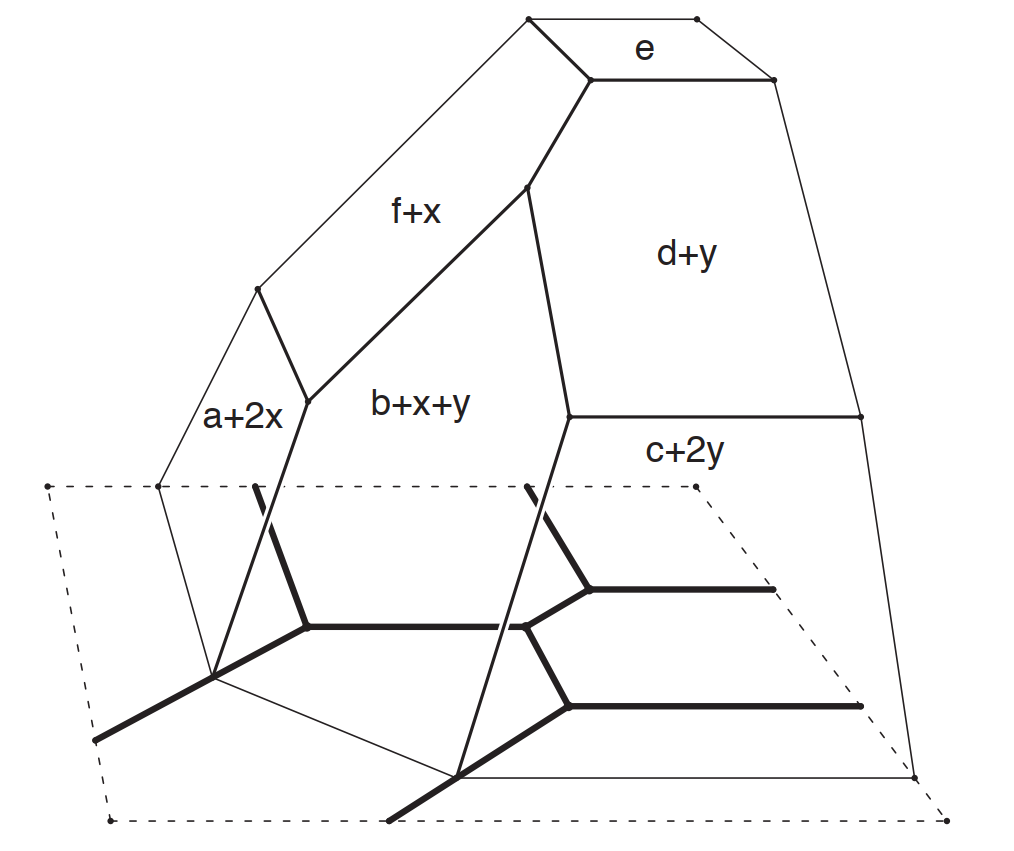
\includegraphics[scale=0.5]{graphics/quad_trop_pol_proj.PNG}
\caption{The graph and the curve defined by a quadratic polynomial.\cite[p.~22]{maclagan2015introduction}}
\label{fig:quad_trop_var}
\end{figure}

To understand the geometry of tropical rational functions, tropical polynomial maps and tropical rational maps better we will show that each are piecewise linear.


\begin{lemma}
Tropical rational functions are piecewise linear functions. Tropical polynomial maps and tropical rational maps are piecewise linear maps.
\end{lemma}
\begin{proof}
Because of lemma \ref{lemma:trop_properties} tropical polynomials are piecewise linear. Tropical division, $\oslash$, is a linear transformation, therefore tropical rational maps are piecewise linear two. Now this means that tropical rational maps and tropical polynomial maps are also piecewise linear and the notion of linear regions applies.
\end{proof}

\begin{definition}\cite[p.~4]{zhang2018tropical}
A \textbf{convex polyhedron} or just \textbf{polyhedron} is a set defined by linear inequalities with integer coefficients:
$$\{x \in \mathbb{R} \ | \ Ax \leq b \}$$
for $A \in \mathbb{Z}^{m \times d}$ and $b \in \mathbb{R}^{m}$. A \textbf{polygon} is a bounded polyhedron.
\end{definition}

\begin{definition}\cite[p.~4]{zhang2018tropical}
\label{def:lin_reg_of}
A \textbf{linear region} of $F \in Rat(d, m)$ is a, with respect to inclusion, maximal connected subset of the domain on which $F$ is linear. The number of linear regions of $F$ is denoted $\mathcal{N}(f)$.
\end{definition}
A linear region as in \ref{def:lin_reg_of} is a polyhedron.
\begin{definition}
A \textbf{face} of a polyhedron $P \subset \mathbb{R}^{n}$ is a subset of the form
$$F= P \cap \{x \in \mathbb{R}^{n} \ | \ c^{t}x = b_0 \}$$
where $c \in \mathbb{R}^{n}$ and $b_0 \in \mathbb{R}$ are picked picked so that
$$P \subset \{ x \in \mathbb{R} \ | \ c^{t}x \leq b_0 \}$$
holds.
\end{definition}

\begin{definition}\cite{maclagan2015introduction}
A \textbf{polyhedral complex} is a collection of polyhedra satisfying two conditions:
\begin{itemize}
\item[(i)]
if a polyhedron $P$ is in the collection, then so is any face of $P$
\item[(ii)]
if $P$ and $Q$ lie in the collection then $P \cap Q$ is a face of both $P$ and $Q$.
\end{itemize}
\end{definition}
\begin{definition}
Let $\Sigma$ be a polyhedral complex and $d \in \mathbb{N}$, then the \textbf{d-skeleton} of $\Sigma$ is the the conjunction of all faces of $\Sigma$ of dimension $\leq d$.
\end{definition}
\begin{definition}\cite{maclagan2015introduction}
The support $\text{supp}(\Sigma)$ of a polyhedral complex $\Sigma$ is the set $\{ x \in \mathbb{R}^{n} \ | \ x \in P \ \text{for some} \ P \in \Sigma \}.$
\end{definition}


The linearity of a tropical polynomial per definition will be broken in its hypersurface and linear everywhere else. Therefore the tropical hypersurface $\mathcal{T}(f)$ of a tropical polynomial $f$ divides the domain of f into convex cells on each of witch f is linear. Tropical hypersurfaces of polynomials in two variables are called \textbf{tropical curves}.\cite[p.~3]{zhang2018tropical}

\begin{definition}
Let $A \subset \mathbb{R}^{n}$ be a real subset with $n \in \mathbb{N}$. Then the set $\Conv(A) = \{\lambda x + (1- \lambda)y \ | \ x, y \in A \ \text{and} \ \lambda \in [0,1] \subset \mathbb{R}\}$ is called the \textbf{convex hull} of $A$.
\end{definition}

\begin{definition}\cite[p.~3]{zhang2018tropical}
The \textbf{Newton polygon} of a tropical polynomial $f(x) = c_1 x^{\alpha_1} \oplus \dots \oplus c_r x^{\alpha_r}$  is the convex hull of $\alpha_1 , \dots , \alpha_r \in \mathbb{N}^{d}$, regarded as points in $\mathbb{R}^{d}$,
$$ \Delta(f) := \Conv\{\alpha_i \in \mathbb{R}^{d} : c_i \neq -\infty , i = 1, \dots ,r \}. $$
\end{definition}

\begin{remark}\cite[p.~3]{zhang2018tropical}
Let $f = c_1 x^{\alpha_1} \oplus \dots \oplus c_r x^{\alpha_r}$ be a tropical polynomial. We first, lift each $\alpha_i$ from $\mathbb{R}^d$ into $\mathbb{R}^{d+1}$ by appending $c_i$ as the last coordinate. Denote the convex hull of the lifted $\alpha_1, \dots , \alpha_r$ as
$$\mathcal{P}(f):= \Conv{(\alpha_i, c_i) \in \mathbb{R}^{d} \times \mathbb{R} : i = 1, \dots , r}.$$
Next let $UF(\mathcal(P)(f))$ denote the collection of upper faces in $\mathcal{P}(f)$ and $\pi : \mathbb{R}^{d} \times \mathbb{R} \to \mathbb{R}^{d}$ be the projection that drops
the last coordinate. The dual subdivision determined by $f$
is then
$$\delta(f) := {\pi(p) \subset \mathbb{R}^{d} : p \in UF( \mathcal{P}(f))}.$$
$\delta (f)$ forms a polyhedral complex with support $\delta (f)$. By \cite[Proposition 3.1.6.]{maclagan2015introduction}, the tropical hypersurface $\mathcal{T}(f)$ is the $(d - 1)$-skeleton of the polyhedral complex dual to $ \delta(f)$. This means that each vertex in $ \delta(f)$ corresponds to one "cell" in $R^{d}$ where the function f is linear. Thus, the number of vertices in $\mathcal{P}(f)$ provides an upper bound on the number of linear regions of $f$.
\end{remark}

Our analysis of neural networks will require figuring out
how the polytope $\mathcal{P}(f)$ transforms under tropical power,
sum, and product.

\begin{proposition}\cite[p.~4]{zhang2018tropical}
Let $f$ be a tropical polynomial and let $a \in \mathbb{N}$, then
$$ \mathcal{P}(f^{a}) = a \mathcal{P}(f).$$
The set $a \mathcal{P}(f) = \{ax : x \in \mathcal{P}(f) \} \subset \mathbb{R}^{d + 1}\}$ is a scaled version of $\mathcal{P}(f)$ with the same shape but different volume.
\end{proposition}
\begin{proof}
Let $f(x)=c_{1}x^{\alpha_1} \oplus \dots \oplus c_{r}x^{\alpha_r}, f:\mathbb{T}^{n} \to \mathbb{T}$, as in definition \ref{def:tropPolyn}. Then with $\mathcal{P}(f) = \Conv\{(\alpha_{i}, c_{i}) \in \mathbb{R}^{d} \times \mathbb{R}, i= 1, \dots , r \ \text{and} \ c_{i} \neq - \infty \}$.
\begin{align*}
f^{a} &= (c_{1}x^{\alpha_{1}} \oplus \dots \oplus c_{r} x^{\alpha_{r}})^{a} \\
&= a \cdot (c_{1}x^{\alpha_{1}} \oplus \dots \oplus c_{r} x^{\alpha_{r}}) \\
&= a \cdot (c_{1}x^{\alpha_{1}}) \oplus \dots \oplus a \cdot (c_{r} x^{\alpha_{r}}) \\
&= (a \cdot c_{1})x^{a \cdot \alpha_{1}} \oplus \dots \oplus (a \cdot c_{r}) x^{a \cdot \alpha_{r}}
\end{align*}
and therefore
$$\mathcal{P}(f^{a}) = \Conv\{(a \cdot \alpha_{i}, a \cdot c_{i}) \in \mathbb{R}^{d} \times \mathbb{R}, i = 1, \dots, r \ \text{and} \ c_{i} \neq - \infty \} = a\mathcal{P}(f)$$.
\end{proof}

A generalisation of normal summation, now on sets, is the Minkowski sum.

\begin{definition}\cite[p.~4]{zhang2018tropical}
The Minkowski sum of two sets $P_1$ and $P_2$ in $\mathbb{R}^{d}$ is the set
$$ P_1 + P_2 := \{x_1 + x_2 \in \mathbb{R}^{d} : x_1 \in P_1 ,x_2 \in P_2 \};$$
and for $\lambda_1 , \lambda_2 \geq 0$, their weighted Minkowski sum is
$$ \lambda_1 P_1 + \lambda_2 P_2 := \{ \lambda_1 x_1 + \lambda_2 x_2 \in \mathbb{R}^{d} : x_1 \in P_1 , x_2 \in P_2 \} $$.
\end{definition}

One important example for an Minkowski sum is a zonotope. For that we need a notion of the following.
\begin{definition}
A subset $A \subset \mathbb{V}$ of a vector space $\mathbb{V}$ is a line segment, if $A=\{\lambda x + \lambda (1-y) \ | \ \lambda \in [0,1]\subset \mathbb{K}\}$ with $\mathbb{K}$ being the scalar field of $\mathbb{V}$.
\end{definition}

\begin{definition}
The Minkowski sum of line segments is called a zonotope.
\end{definition}

\begin{definition}
\label{def:point_sym}
Let $A \subset \mathbb{R}^{n}$ be a set. A is point symmetric around $b \in A$ if for $a \in A$ follows $a + 2(b-a)=2b-a \in A$
\end{definition}

Obviously for $A$ and $b$ as in definition \ref{def:point_sym} and if $A$ is convex, then $b \in A$ the symmetry point must lie in $A$. We build an intuition of zonotopes by proving the following statement.

\begin{lemma}
\label{lem:zon_sym_conv}
A zonotope over $\mathbb{R}^{n}$ is point symmetric and convex.
\end{lemma}
\begin{proof}
We proof a zonotope is point symmetric and convex by induction. As base case let $P \subset \mathbb{R}^{n}$ be a line segment in between $x, y \in \mathbb{R}^{n}$ then $P$ is obviously point symmetric around $b=0.5(x+y) \in \mathbb{R}^{n}$ and convex per definition. For the induction step let $A \subset \mathbb{R}^{n}$ be a convex set and point symmetric around $b \in \mathbb{R}^{n}$ and also let $P = \{ \lambda x + (1- \lambda) y | \lambda \in [0,1] \subset \mathbb{R}^{n} \}$ for $x, y \in \mathbb{R}^{n}$. Then the Minkowski sum of the two sets is
\begin{align*}
A + P 
&= \{ a + p \ | \ a \in A \ \text{and} \ p \in P \} \\
&= \{ a + \lambda x + (1- \lambda) y \ | \ a \in A \ \text{and} \ \lambda \in [0,1] \}
\end{align*}
It follows that $a_{A+P} \in A+P$ has the form $a_{A+P}=a + \lambda x + (1- \lambda)y$ for $a\in A$ and $\lambda \in [0,1]$. We set $b_{A+P}=(0.5)(x+y) + b$. Then
\begin{align*}
a_{A+P} &+ 2(b_{A+P} - a_{A+P}) \\
&= a + \lambda x + (1- \lambda)y + 2( 0.5(x+y) + b - (a + \lambda x + (1-\lambda)y)) \\
&= 2b-a + (1- \lambda) x + \lambda y \in A+P
\end{align*}
since $2b-a \in A$ and $(1- \lambda) x + \lambda y \ \in P$. Therefore a zonotope is symmetric.
Similarly for convexity let $p, q \in A+P$ have the shape
\begin{align*}
p &= a_{p} + \lambda_{p} x + (1 - \lambda_{p}) y \\
q &= a_{q} + \lambda_{q} x + (1 - \lambda_{q}) y.
\end{align*}
For $\mu \in [0, 1] \subset \mathbb{R}^{n}$ we need to compute
\begin{align*}
\mu p + (1 - \mu) q &= \mu (a_{p} + \lambda_{p} x + (1-\lambda_{p}) y) + (1-\mu)(a_{q} + \lambda_{q} x + (1-\lambda_{q}) y) \\
&= \mu a_{p} + (1-\mu) a_{q} + (\mu \lambda_{p} + (1-\mu)\lambda_{q})x + (\mu(1-\lambda_{p}) + (1-\mu)(1-\lambda_{q}))y \\
&= \mu a_{p} + (1-\mu) a_{q} + \Phi x + (1- \Phi) y
\end{align*}
with $\Phi = \Phi(\mu , \lambda_{p}, \lambda_{q}) = \mu \lambda_{p} + \lambda_{q} - \mu \lambda_{q}$. If $0 \leq \Phi (\mu, \lambda_{p}, \lambda_{q}) \leq 1$, then a zonotope would be convex, since $(1-\mu) a_{q} + \Phi x + (1- \Phi) y \in P$ would hold and $\mu a_{p} + (1-\mu) a_{q} \in A$ holds anyway. So to conclude we show $0 \leq \Phi (\mu, \lambda_{p}, \lambda_{q}) \leq 1$. \
Because of $\mu \lambda_{p} \geq 0$ and $\lambda_{q} \geq \mu \lambda_{q}$ follows $\Phi \geq 0$. $\Phi$ is maximal for $\lambda_{p} = 1$ and $\Phi (\mu, 1, \lambda_{q}) = \mu + \lambda_{q} - \mu \lambda_{q} \leq 1$.
\end{proof}

Let $\mathcal{V}$ denote the set of vertices of a polytope $P$. Clearly, the Minkowski sum of two polytopes is given by the convex hull of the Minkowski sum of their vertex sets, i.e., $P_{1} + P_{2} = \Conv(\mathcal{V}(P1) + \mathcal{V}(P2))$. With this observation, the
following is immediate.

\begin{proposition} \cite[p.~4]{zhang2018tropical}
Let $f, g \in Pol(d, 1) = \mathbb{T}[x_1, \dots , x_d]$ be tropical polynomials. Then
\begin{align*}
\mathcal{P}(f \odot g) &= \mathcal{P}(f) + \mathcal{P}(g), \\
\mathcal{P}(f \oplus g) &= \Conv(\mathcal{V}(\mathcal{P}(f)) \cup \mathcal{V}( \mathcal{P}(g))).
\end{align*}
\end{proposition}

We reproduce below part of \cite[Theorem 2.1.20]{gritzmann1993minkowski} and derive a corollary for bounding the number of verticies on the upper faces of a zonotope.

\begin{theorem}
\label{theo:gritzmann_sturmfels}
\cite{gritzmann1993minkowski}. Let $P_1, \dots , P_k$ be polytopes in $\mathbb{R}^{d}$ and let m denote the total number of nonparallel edges of $P_1, \dots , P_k$. Then the number of vertices of $P_1 + \dots + P_k$ does not exceed
$$\sum_{j=0}^{d-1} \binom{m-1}{j}.$$
The upper bound is attained if all $P_i$'s are zonotopes and all their generating line segments are in general positions.
\end{theorem}

And now we come to the main corollary of this chapter, core to chapter \ref{sec:tropical_geometry_of_neural_networks}.

\begin{corollary}\cite[p.~4]{zhang2018tropical}
Let $\mathcal{P} \in \mathbb{R}^{d+1}$ be a zonotope generated by m line segments $P_1 , \dots , P_m$. Let $\pi : \mathbb{R}^{d} \times \mathbb{R} \to \mathbb{R}^{d}$ be the projection. Suppose $P$ satisfies:
\begin{itemize}
\item[(i)]
the generating line segments are in general positions;
\item[(ii)]
the set of projected vertices $\{ \pi(v) : v \in \mathcal{V}(\mathcal{P}) \} \subseteq \mathbb{R}^{d}$ are in generalposition.
\end{itemize}
Then $P$ has
$$ \sum_{j=0}^{d} \binom{m}{j} $$
vertices on its upper faces. If either (i) or (ii) is violated, then this becomes an upper bound.
\end{corollary}
\begin{proof}
Let $V_{1}$ be the vertices of the upper and $V_{2}$ the vertices of the lower face of P in relation to the projection $\pi$. As a consequence of (i), $P_{1}, \dots , P_{k}$ are nonparallel and with \ref{theo:gritzmann_sturmfels} follows the number of vertices of $\mathcal{P}$ is 
$$n_{1} = 2 \sum^{d}_{j=0} \binom{m-1}{j}.$$ 
Because a zonotope is convex \ref{lem:zon_sym_conv} the upper and lower faces of P must already be all faces and $|V_{1} \cup V_{2}| = n_{1}$ holds. Also because of \ref{lem:zon_sym_conv}, zonotopes are symmetric and therefore $|V_{1}| = |V_{2}|$ the upper and lower faces are of same cardinality. Let $P' := \pi (P)$ be the projection of $P$ in $\mathbb{R}^{d}$. (ii) would not hold if $\pi(P_{1}), \dots , \pi(P_{2})$ where not in general position and therefore $P'$ is generated by m line segments and $P'$ has 
$$n_{2}=2 \sum^{d-1}_{j=0} \binom{m-1}{j}$$
vertices, since the dimension has gone one lower. For any vertex $v \in P$, if $v \in V_{1} \setminus V_{2} \cup V_{2} \setminus V_{1}$ then $v$ can not be a vertex of $P'$ since all of these get dropped by the projection. On the other hand $v \in (V_{1} \cup V_{2}) \setminus (V_{1} \setminus V_{2} \cup V_{2} \setminus V_{1}) = V_{1} \cap v_{2}$ can not get dropped by the projection of $P$ and therefore the number of vertices on $P'$ equals $|V_{1} \cap V_{2}|$, thus $n_{2} = |V_{1} \cap V_{2}|$ and we can calculate the number of vertices on the upper face of $P$:
\begin{align*}
|V_{2}|
&= 0.5(|V_{1} \cup V_{2}| - |V_{1} \cap V_{2}|) + |V_{1} \cap V_{2}| \\
&= 0.5(n_{1} - n_{2}) + n_{2} \\
&= 0.5(2 \sum^{d}_{j=0} \binom{m-1}{j} - 2 \sum^{d-1}_{j=0} \binom{m-1}{j}) + 2 \sum^{d-1}_{j=0} \binom{m-1}{j} \\
&= \binom{m-1}{d} + 2 \sum^{d-1}_{j=0} \binom{m-1}{j} \\
&= \sum^{d}_{j=0}(\binom{m-1}{j} + \binom{m-1}{j-1}) \\
&= \sum^{d}_{j=0} \binom{m}{j}
\end{align*}
\end{proof}

\newpage

\section{Tropical geometry of neural networks}
\label{sec:tropical_geometry_of_neural_networks}

\begin{remark}\cite{zhang2018tropical}
As explained in remark \ref{rem:score_fkt}, a neural network $\nu : \mathbb{R}^{d} \to \mathbb{R}^{p}$ together with a choice of score function $s : \mathbb{R}^{p} \to \mathbb{R}$ give us a classifier. If the output value $s(\nu(x))$ exceeds some
decision threshold $c$, then the neural network predicts $x$ is
from one class (e.g., $x$ is a CAT image), and otherwise $x$
is from the other category (e.g., a DOG image). The input
space is thereby partitioned into two disjoint subsets by the
\textbf{decision boundary} $\mathcal{B} = \{ x \in \mathbb{R}^{d}: \nu(x)=s(c)^{-1} \}$. Connected regions with value above the threshold and connected
regions with value below the threshold will be called the
\textbf{positive regions} and \textbf{negative regions} respectively.
\end{remark}

\begin{proposition}\cite{zhang2018tropical}(Tropical geometry of decision boundary).
Let $v : \mathbb{R}^{d} \to \mathbb{R}$ be an $L$-layer neural network satisfying assumptions (a)–(c) with $t^{L}=-\infty$. Let the score function $s: \mathbb{R} \to \mathbb{R}$ be injective with decision threshold $c$ in its range. If $v = f \oslash g$ where $f$ and $g$ are tropical polynomials, then \\
(i) its decision boundary $\mathcal{B}=\{ x \in \mathbb{R}^{d} : v(x) = s^{-1}(c)\}$ divides $\mathbb{R}^{d}$ into at most $\mathcal{N} (f)$ connected positive regions and at most $\mathcal{N}(g)$ connected negative regions; \\
(ii) if $c \in \mathbb{R}$ is such that there is no tropical monomial in $f(x)$ that differs from any tropical monomial in $g(x)$ by $c$, then its decision boundary is contained in the tropical hypersurface of the tropical polynomial $s^{-1}(c) \odot g(x) \oplus f(x) = \max\{f(x), g(x) + s^{-1}(c)\}$, i.e.,
$$\mathcal{B} \subseteq \mathcal{T} (s^{-1}(c) \odot g \oplus f).$$
\end{proposition}
\begin{proof}
For the first statement let $s^{-1}(c)=c' \in \mathbb{R}$ and $U_1 , \dots , U_{\mathcal{N}(f)}$ be the regions of $\mathbb{R}^{d}$ on which $f$ is linear. Each of the $U_i$ is convex for $i=1 , \dots , \mathcal{N}(f)$ since if we take two elements from $U_i$, then all elements on the connecting line segment also have to have the same maximal monomial, or else the initial elements would have had different maximal monomials. Because of lemma \ref{lemma:trop_properties} the tropical monomial $-g$ will be concave on $U_i$ for $i = 0 1, \dots , \mathcal{N}(f)$ and with
\begin{align*}
(f \oslash g) (\lambda x + (1-\lambda)y)
&= \lambda f(x) + (1-\lambda) f(y) - g(\lambda x + (1-\lambda)y) \\
&\geq \lambda (f \oslash g)(x) + (1-\lambda) (f \oslash g) (y)
\end{align*}
for all $x, y \in U_i$ and $\lambda \in [0,1] \subset \mathbb{R}$ the tropical rational function $f \oslash g$ will also be concave on $U_i$. Now because $f \oslash g$ are concave on $U_i$, with them selves are convex we can show that the set $\{x \in U_i : f \oslash g(x) \geq c'$ must be convex:
\begin{align*}
(f \oslash g) (\lambda x + (1-\lambda)y)
&= \lambda f(x) + (1-\lambda) f(y) - g(\lambda x + (1-\lambda)y) \\
&\geq \lambda (f \oslash g)(x) + (1-\lambda) (f \oslash g) (y) \\
&\geq \lambda c + (1-\lambda)c \\
&= c.
\end{align*}
If there where disjunct connected positive regions then $\{ x \in U_i : (f \oslash g)(x) \geq c' \}$ would not be convex and therefore there can only be one connected positive region on $U_i$ for $i = 1, \dots , \mathcal{N}(f)$. \\
Now if we divide $\mathbb{R}^{d}$ in to $\mathcal{N}(g)$ convex regions on which $g$ is linear, then $f \oslash g$ is convex on these regions and $\mathcal{N}(g)$ holds as upper bound to the connected negative regions in the save way. \\
For the second statement we rearange the terms in the decision boundary $\mathcal{B} = \{ x \in \mathbb{R}^{d} : \nu(x) = s^{-1}(c) \} = \{ x \in \mathbb{R}^{d} : f(x) = g(x) + c' \}$ and since $f(x)$ and $g(x) + c'$ are both tropical polynomial, we have
\begin{align*}
f(x) &= b_1 x{\alpha_1} \oplus \dots \oplus b_r^{\alpha_r}, \\
g(x) + c &= c_1 x^{\beta_1} \oplus \dots \oplus c_s x^{\beta_s},
\end{align*}
with appropriate multiindices $\alpha_1 , \dots , \alpha_r, \beta_1 , \dots , \beta_s$, and real coefficients $b_1, \dots , b_r, c_1, \dots , c_s$. By the assumption on
the monomials, we have that $x_0 \in \mathcal{B} $ only if there exist $i, j$ so that $\alpha_i \neq \beta_j$ and $b_i x_0^{\alpha_i}$. This completes the proof since if we combine the monomials of $f{x}$ and $g(x) + c$ by (tropical) summing them into a single tropical polynomial, $\max \{f(x), g(x) + c\}$, the above implies that on the level set, the value of the combined tropical polynomial is attained by at least two monomials and therefore $x_0 \in \mathcal{\max\{f(x), g(x) + c\}}$.
\end{proof}

\begin{theorem}\cite[p.~8]{zhang2018tropical}
\label{theo:lin_reg}
Let $\nu : \mathbb{R}^{d} \to \mathbb{R}$ be an $L$-layer real-valued feedforeard neural network satisfying (a)-(c). Let $t^{(L)}=-\infty$ and $n_{l} \geq d$ for all $l=1, \dots , L-1$. Then $\nu = \nu^{(L)}$ has at most
$$\displaystyle\prod^{L-1}_{l=1}\displaystyle\sum^{d}_{i=0}\binom{n_l}{i}$$
linear regions. In particular, if $d \leq n_1, \dots , n_{L-1} \leq n$, the number of linear regions of $\nu$ is bounded by $\mathcal{O}(n^{d(L-1)})$.
\end{theorem}

The rest of section \ref{sec:tropical_geometry_of_neural_networks} will be devoted the proof of theorem \ref{theo:lin_reg}.

\begin{definition}\cite[p.~15]{zhang2018tropical}
Given a tropical rational map $F \in \Rat(d, m)$, we define $\mathcal{T}(F)$ to be the boundaries between adjacent linear regions. When $F=(f_1, \dots , f_m) \in \Pol(d, m)$, i.e., a tropical polynomial map, this set is exactly the union of tropical hypersurfaces $\mathcal{T}(f_i), i=1, \dots , m$. Therefore this definition of $\mathcal{T}(F)$ extends Definition \ref{def:trop_hyper}.
\end{definition}

When restricting a function $f: X \to Y$ on the domain $C \subset X$ we will write $\restr{f}{C}$ for the restriction $\restr{f}{C} : C \to Y$.

\begin{definition}
The convex degree of a tropical rational map $F \in \Rat(d,n)$ is the minimum division of $\mathbb{R}^{d}$ into convex
regions over which $F$ is linear, i.e.
$$\mathcal{N}_{C}(F) := \min\{n:C_1 \cup \dots \cup C_n = \mathbb{R}^{d} \ \text{where} \ C_i \ \text{convex and} \ \restr{F}{C_i} \ \text{linear}\}.$$
\end{definition}

\begin{definition}
\label{def:conv_deg_restr}
For $m \leq d$ and $F \in \Rat(d,n)$, we will denote by $\mathcal{N}_{C}(F \ | \ m)$ the maximum convex degree obtained by restricting $F$ to an $m$-dimensional affine subspace in $\mathbb{R}^{d}$, i.e.,
$$\mathcal{N}_C(F \ | \ m) := \max \{ \mathcal{N}_C(\restr{F}{\Omega}): \Omega \subseteq \mathbb{R}^{d} \ \text{is an} \ m \text{-dimensional affine space} \}.$$
\end{definition}

We will use the convention, that if $m > d$ and $F$ as in definition \ref{def:conv_deg_restr} then $\mathcal{N}_C(F \ | \ m) = \mathcal{N}_C(F)$.

\begin{definition}
Consider a tropical rational map $F=(f_1, \dots , f_n) \in \Rat(d, n)$ and $\alpha = (a_1, \dots , a_n) \in \mathbb{Z}^{d}$. Then we define following notation:
$$F^{\alpha} := \alpha^{T} F = a_1 f_1 , \dots , a_n f_n = \displaystyle\bigodot_{i=1}^{n} a_i f_i \in \Rat(d, 1).$$
\end{definition}

\begin{definition}
Let $f: X \to Y$ be a function. Then the \textbf{Image} of $f$ is the subset $\text{Im}(f) = \{f(x) : x \in X\} \subset Y$.
\end{definition}

\begin{definition}
\label{def:gen_exp}
$\alpha = (a_1, \dots, a_n) \in \mathbb{Z}^{n}$ is said to be a general exponent of $F \in \Rat(d, n)$ if the linear regions of $F^{\alpha}$ and the linear regions of $F$ are identical.
\end{definition}

\begin{lemma}
Let $F \in \Rat(d, n)$. Then
\begin{itemize}
\item[(i)]
$\mathcal{N}(F^{\alpha}) = \mathcal{N}(F)$ if and only if $\alpha$ is a general exponent;
\item[(ii)]
$F$ has a general exponent $\alpha \in \mathbb{N}^{n}$.
\end{itemize}
\end{lemma}
\begin{proof}
First we proof (i). From definition \ref{def:gen_exp} follows that $\alpha$ is in general position if the linear regions of $F$ and $F^{\alpha}$ are identical. If the linear regions are identical, the points $x \in \mathbb{R}^{d}$ at which linear regions meat and therefore where $F$, $F^{\alpha}$ are not differentiable are identical. It directly follows that $\mathcal{T}(F^{\alpha})=\mathcal{T}(F) \subset \mathbb{R}^{d}$ are identical and in conclusion the number of linear regions $\mathcal{N}(F^{\alpha}) = \mathcal{N}(F)$ must also be identical. \\
For (ii) we need analytical basics, that we will not introduce extensively, but rather refer the reader to \cite{tao2016analysis}. We need to show that there always exists an $\alpha \in \mathbb{N}^{\alpha}$ such that $F^{\alpha}$ divides its domain $\mathcal{R}^{d}$ into the same set of linear regions as $F$. In other words, for every pair of adjacent linear regions of $F$, the faces in $\mathcal{T}(F)$ that separates them is also present in $\mathcal{T}(F^{\alpha})$. \\
Let $L$, $M$ be adjacent linear regions of $F$. Then $\restr{F}{L}$ and $\restr{F}{M}$ are tropical monomials where for instance $\restr{F}{L}$ has the form
$$\restr{F}{L}(x) = \begin{bmatrix}
c_1 \odot x^{\alpha_1} \\ \vdots \\ c_n \odot x^{\alpha_n}
\end{bmatrix} = \begin{bmatrix}
c_1 + \alpha_{11} x_1 + \dots + \alpha_{1d}x_d \\
\vdots \\
c_n + \alpha_{n1} x_1 + \dots + \alpha_{nd}x_d
\end{bmatrix}
$$
and therefore the differential is of the form:
$$d\restr{F}{L} = \begin{bmatrix}
\alpha_{11} & \cdots & \alpha_{1d} \\
\vdots & \ddots & \vdots \\
\alpha_{n1} & \cdots & \alpha_{nd}
\end{bmatrix}.$$
We see that the differentials of $\restr{F}{L}, \restr{F}{M}$ must have integer coefficients $d\restr{F}{L}, d\restr{F}{M} \in \mathbb{Z}^{nd}$ and also be $d\restr{F}{L} \neq d\restr{F}{M}$ unequal, because otherwise $L$ and $M$ can be merged into a single region. With that in mind it is clear, that $Im(d\restr{F}{L} - d\restr{F}{L}) \neq \{0\}$ and the solutions set $\{\alpha \in \mathbb{N}^{n} : (\restr{F}{L} - d\restr{F}{L})^{T}\alpha = 0\}$ is of dimension $\geq 1$. With the observation that $d\restr{F^{\alpha}}{L} = \alpha^{T}d\restr{F}{L}$:
$$d\restr{F^{\alpha}}{L} = \begin{bmatrix}
\alpha_1 a_{11} + \dots + \alpha_n a_{n1} \\
\vdots \\
\alpha_1 a_{1d} + \dots + \alpha_n a_{nd}
\end{bmatrix} = \begin{bmatrix}
\alpha_1 \\
\vdots \\
\alpha_n
\end{bmatrix}^{T}
\cdot \begin{bmatrix}
 a_{11} + \dots + a_{n1} \\
\vdots \\
a_{1d} + \dots + a_{nd}
\end{bmatrix}
= \alpha^{T}d\restr{F}{L},$$
and the same holds for $d\restr{F^{\alpha}}{M}$. We set $\mathcal{A}(F)$ to be the collection of all pairs of adjacent linear regions of $F$, this set is finite. Since the set of $\alpha$ that degenerates two adjacent linear regions into a single one, i.e.,
$$\mathcal{S} := \displaystyle\bigcup_{(L,M) \in \mathcal{A}(F)}\{\alpha \in \mathbb{N}^{n} : (d\restr{F}{L} - d\restr{F}{M})^{T}\alpha=0\},$$
is contained in a union of a finite number of hyperplanes in $\mathbb{R}^{n}$, $\mathcal{S}$ cannot cover the entire lattice of nonnegative integers $\mathbb{N}^{n}$.
Therefore the set $\mathbb{N}^{n} \cap (\mathbb{R}^{n} \setminus \mathcal{S})$ is nonempty and any of its element is a general exponent for $F$.
\end{proof}

\begin{theorem}
Let $F=(f_1, \dots , f_m) \in \Rat(n,m)$ and $G \in \Rat(d, n)$. Define $H = (h_1, \dots , h_m) \in \Rat(d, m)$ by
$$h_i := f_i \circ G, \ \ i=1, \dots , m.$$
Then
$$\mathcal{N}(H) \leq \mathcal{N}_{C}(H) \leq \mathcal{N}_C(F \ | \ d) \cdot \mathcal{N}_C(G).$$
\end{theorem}
\begin{proof}
The first inequality holds because the regions we are counting in $\mathcal{N}_{C}(H)$ have one more restraint than the regions that are counted in $\mathcal{N}(H)$, that they have to be convex, and there fore $\mathcal{N}(H) \leq \mathcal{N}_{C}(H)$. For the second inequality we know by the definition of $\mathcal{N}_C(G)$ that there exist convex sets $C_1, \dots , C_{\mathcal{N}_C(G)}$ whose union is $\mathbb{R}^{d}$ and on each of which $G$ is linear. So $\restr{G}{C_i}$ is some affine function $\rho_i$. Now we want to show for $i = 1, \dots, \mathcal{N}_C(G)$ that $\mathcal{N}_C(F \circ \rho_i) \leq \mathcal{N}_C(F \ | \ d)$ and first remind of the definitions:
\begin{align*}
\mathcal{N}_{c}&(F \circ \rho_i) = \min\{n : C_1 \cup \dots \cup C_n = \mathbb{R}^{d} \ \text{where} \ C_i \ \text{convex and} \ \restr{F \circ \rho_i}{C_i} \ \text{linear}\} \\
&\leq \mathcal{N}_C(F \ | \ d) = \max\{\mathcal{N}_C(\restr{F}{\Omega}) : \Omega \subset \mathbb{R}^{n} \ \text{is an} \ d \ \text{dimensional affine space} \}.
\end{align*}
The set $\text{Im}(\rho_i) \subset \mathbb{R}^{n}$ is a linear subspace, which also is an affine space. If $d < n$ then the Image of $\rho$, $\text{Im}(\rho_i) \subset \mathbb{R}^{n}$ is a $d$-, or lower, dimensional affine space and therefore 
$$\mathcal{N}_C(F \circ \rho_i) \leq \mathcal{N}_C(F \ | \ d).$$ 
On the other hand if $d \geq n$, then 
$$\mathcal{N}_C(F \ | \ d) = \mathcal{N}_C(F \ | \ n) = \mathcal{N}_C(F)$$ 
and $\text{Im}(\rho_i)$ is a linear subspace, combined with the convexity of the $C_i$
$$\mathcal{N}_C(F \circ \rho_i) \leq \mathcal{N}_C(F \ | \ d).$$
holds. Since $F \circ G = F \circ \rho_i$ on $C_i$, we have
$$\mathcal{N}_C(F \circ G) \leq \displaystyle\sum_{i=1}^{k} \mathcal{N}_C(F \circ \rho_i).$$
Hence
$$\mathcal{N}_C(F \circ G) \leq \displaystyle\sum_{i=1}^{k} \mathcal{N}_C(F \circ \rho_i) \leq \displaystyle\sum_{i=1}^{k} \mathcal{N}_C(F \ | \ d) = \mathcal{N}_C(F \ | \ d) \cdot \mathcal{N}_C(G).$$
\end{proof}
\begin{lemma}
Let $\sigma^{(l)} \circ \rho^{(l)}: \mathbb{R}^{n_{l-1}} \to \mathbb{R}^{n_l}$ where $\sigma^{(l)}$ and $\rho^{(l)}$ are affine transformations and activation of the $l$-th layer of a neural network. If $d \leq n_l$, then
$$\mathcal{N}_C(\sigma^{(l)} \circ \rho^{(l)} \ | \ d) \leq \displaystyle\sum_{i=0}^{d}\binom{n_l}{i}.$$
\end{lemma}

\begin{theorem}
Let $\nu : \mathbb{R}^{d} \to \mathbb{R}^{n_L}$ be an $L$-layer neural network satisfying assumptions (a)-(c) with $F^{(l)}$, $G^{(l)}, H^{(l)}$, and $\nu^{(l)}$ as defined in the proof of theorem \ref{teo:trop_char_of_neur_net}. Let $n_l \geq d$ for all $l= 1, \dots , L$. Then
$$\mathcal{N}_C(\nu^{(1)}) = \mathcal{N}_C(G^{(1)}) = \mathcal{N}_C(H^{(1)}) = 1$$
and
$$\mathcal{N}_C(\nu^{(1+1)}) \leq \mathcal{N}_C(\nu^{(1)}) \cdot \displaystyle\sum_{i=0}^{d}\binom{n_{l+1}}{i}.$$
\end{theorem}
\begin{proof}

\end{proof}

\newpage

%%%%%%%%%%%%%%%%%%%%%%%%%%%%%%%%%%
%\tikzset{%
%  every neuron/.style={
%    circle,
%    draw,
%    minimum size=1cm
%  },
%  neuron missing/.style={
%    draw=none, 
%    scale=3,
%    text height=0.333cm,
%    execute at begin node=\color{black}$\vdots$
%  },
%}
%
%\begin{tikzpicture}[x=1.5cm, y=1.5cm, >=stealth]
%
%\foreach \m/\l [count=\y] in {1,2,3,missing,4}
%  \node [every neuron/.try, neuron \m/.try] (input-\m) at (0,2.5-\y) {};
%
%\foreach \m [count=\y] in {1,missing,2}
%  \node [every neuron/.try, neuron \m/.try ] (hidden-\m) at (2,2-\y*1.25) {};
%
%\foreach \m [count=\y] in {1,missing,2}
%  \node [every neuron/.try, neuron \m/.try ] (output-\m) at (4,1.5-\y) {};
%
%\foreach \l [count=\i] in {1,2,3,n}
%  \draw [<-] (input-\i) -- ++(-1,0)
%    node [above, midway] {$I_\l$};
%
%\foreach \l [count=\i] in {1,n}
%  \node [above] at (hidden-\i.north) {$H_\l$};
%
%\foreach \l [count=\i] in {1,n}
%  \draw [->] (output-\i) -- ++(1,0)
%    node [above, midway] {$O_\l$};
%
%\foreach \i in {1,...,4}
%  \foreach \j in {1,...,2}
%    \draw [->] (input-\i) -- (hidden-\j);
%
%\foreach \i in {1,...,2}
%  \foreach \j in {1,...,2}
%    \draw [->] (hidden-\i) -- (output-\j);
%
%\foreach \l [count=\x from 0] in {Input, Hidden, Ouput}
%  \node [align=center, above] at (\x*2,2) {\l \\ layer};
%
%\end{tikzpicture}
%%%%%%%%%%%%%%%%%%%%%%%%%%%%%%%%%%%%%

%\newpage

%\bibliographystyle{amsalpha}
%\bibliography{biblio}{}

%\bibliographystyle{apacite}
%\bibliography{references}

\bibliographystyle{amsalpha}
\bibliography{references}

\end{document}